\chapter{Results and Discussion}\label{ch:results-and-discussion}

\mycomment{
  * Chapter introduction
  * Results section
    > simulate a manual transcriber correcting results by ordering utterances using some metric and using specific WER caclulation
    > Run as average for single conversations AND whole corpus
    > present results using word-confidence
    > could make a table to show percentage of data checked versus reduction in WER?
  * Discussion section
    > average_logprob and utterance confidence are similar- appear to function well for average convo but poorly for whole corpus
    > explain: utterance confidence is calculated from the same logit data as utterance confidence (thus have similar shape)
    > explain word-confidence
    > works much better - long utterances can have few low-confidence words but get high average, word-confidence ordering eliminates this
    > word-confidence seems to work! there is benefit from using this metric
    > other two not so much
    > is this test representative of a real user?
    > by showing that there is a confidence metric which seems to work, Whisper is demonstrated to be a viable choice for aiding a human transcriber
    > perhaps work through requirements?
  * Future work (maybe a better title?)
    > try different type of confidence scoring - perhaps Whisper isn't the best candidate due to the way it makes choices?
    > try different datasets - LifeLUCID is only one out of thousand of corpora, try to replicate results
    > make fully-working transcription software - my example only shows the effect of ordering results, doesn't allow input
    > compare the effect of different model sizes - errors may be clustered differently - if smaller models could reliably get confidence then the hardware and time required to generate transcripts would be minimised
}

\section{Simulating Computer-Aided Transcription}

An effective computer-aided transcription system must reduce the human cost required to lower the amount of errors a transcription to an acceptable level.
By ordering transcribed utterances using some confidence metric and letting a human transcriber make corrections, an effective system should see the error rate fall more rapidly than if the results were corrected in a random order. \\

A simple simulation was devised in order to test the effectiveness of each potential measure of system confidence by using the formula for WER as follows;

\begin{enumerate}
  \item For a set of $M$ utterances $U = \{ u_{0}, u_{1}, \ldots\, u_{M} \}$ (either a single conversation or entire corpus), the subsitutions ($S_i$), deletions ($D_i$), insertions ($I_i$), and number of words in the reference ($N_i$) are calculated for each utterance, $u_i$.
  \item $U$ is ordered using a confidence metric.
  \item The WER, $w_i$, is calculated for a slice of $U$ containing all items including and following some utterance, $u_i$;
    \[
      w_i = \frac{\sum_{j=i}^{M} (S_j + D_j + I_j)}{\sum_{k=0}^{M} N_k}
    \]
  \item Increment $i$ by $1$ then repeat the previous step for all $0 \leq i \leq M$.
    Notice that the denominator is the same for all slices but the numerator changes to simulate each utterance being corrected in order.
  \item Output is a set $W = \{ w_{0}, w_{1}, \ldots\, w_{M} \}$, where some item $w_{i}$ is equal to the WER of $U$ after correcting all utterances prior to $u_i$.
\end{enumerate}

These results shall be analysed by plotting graphs of WER against the percentage of utterance which have been human-corrected, henceforth refered to as 'Cost'.

\section{Simulation Results}

This section details the results acquired from running this simple simulation using results ordered with each of the following metrics;

\begin{itemize}
  \item \texttt{avg\_logprob} taken directly from Whisper's standard output;
  \item utterance-average confidence score; and
  \item utterance-minimum and -maximum word-confidence scores.
\end{itemize}

Where \say{utterance-minimum and -maximum word-confidence} refers to an ordering of utterances based on each utterances minimum and maximum word-level confidence score.

Results which show a per-conversation average have a shaded section to show the standard deviation from the mean, where the mean is the coloured line on the graph.

Dashed 'random order' lines show the WER/Cost trend expected if the results were manually corrected in a random order.
A performant metric for ordering results should have a plot showing a line which dips below the 'random order' line.
A metric which follows the trend of the 'random order' line is thus performing the same as if the results were randomly ordered and therefore ineffective for computer-aided transcription.

\clearpage
\subsection{Utterance-average confidence versus \texttt{avg\_logprob}}\label{subsec:conf-vs-lprob}

\begin{figure}[h!]
 \caption{Per-conversation average WER when evaluating in non-descending order of utterance \texttt{avg\_logprob}}
 \label{fig:average-avg-logprob}
 \centering
 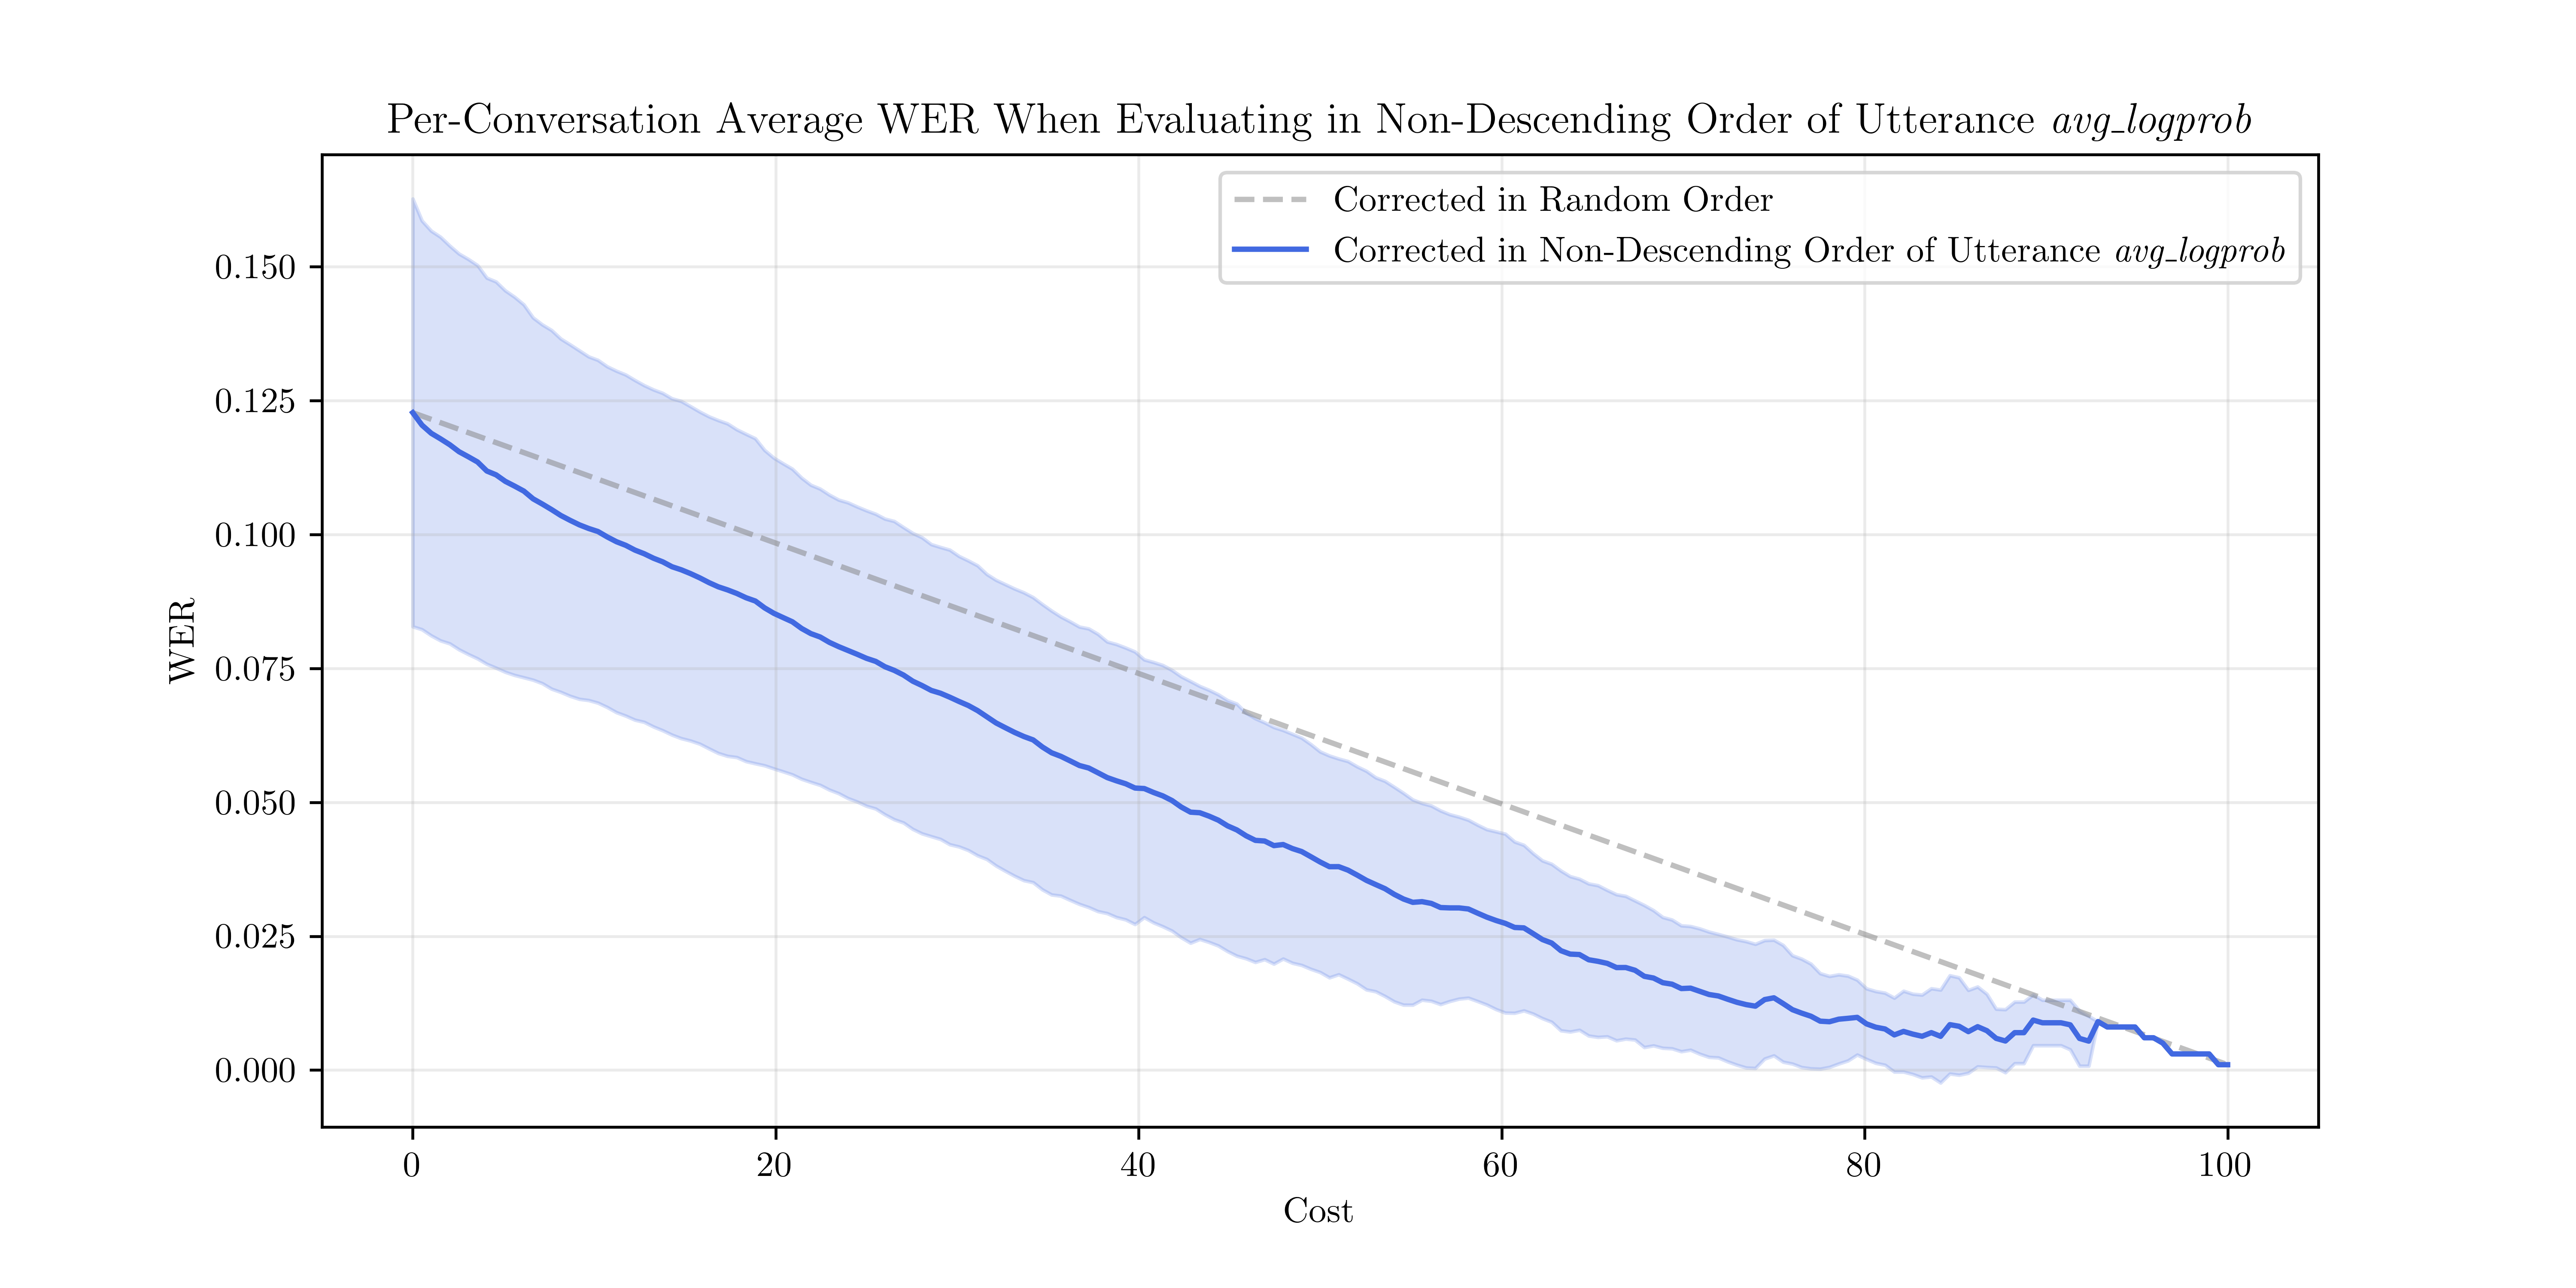
\includegraphics[width=\textwidth]{figures/average-avg-logprob.png}
\end{figure}
\begin{figure}[h!]
 \caption{Per-conversation average WER when evaluating in non-descending order of utterance-average confidence}
 \label{fig:average-uttconf}
 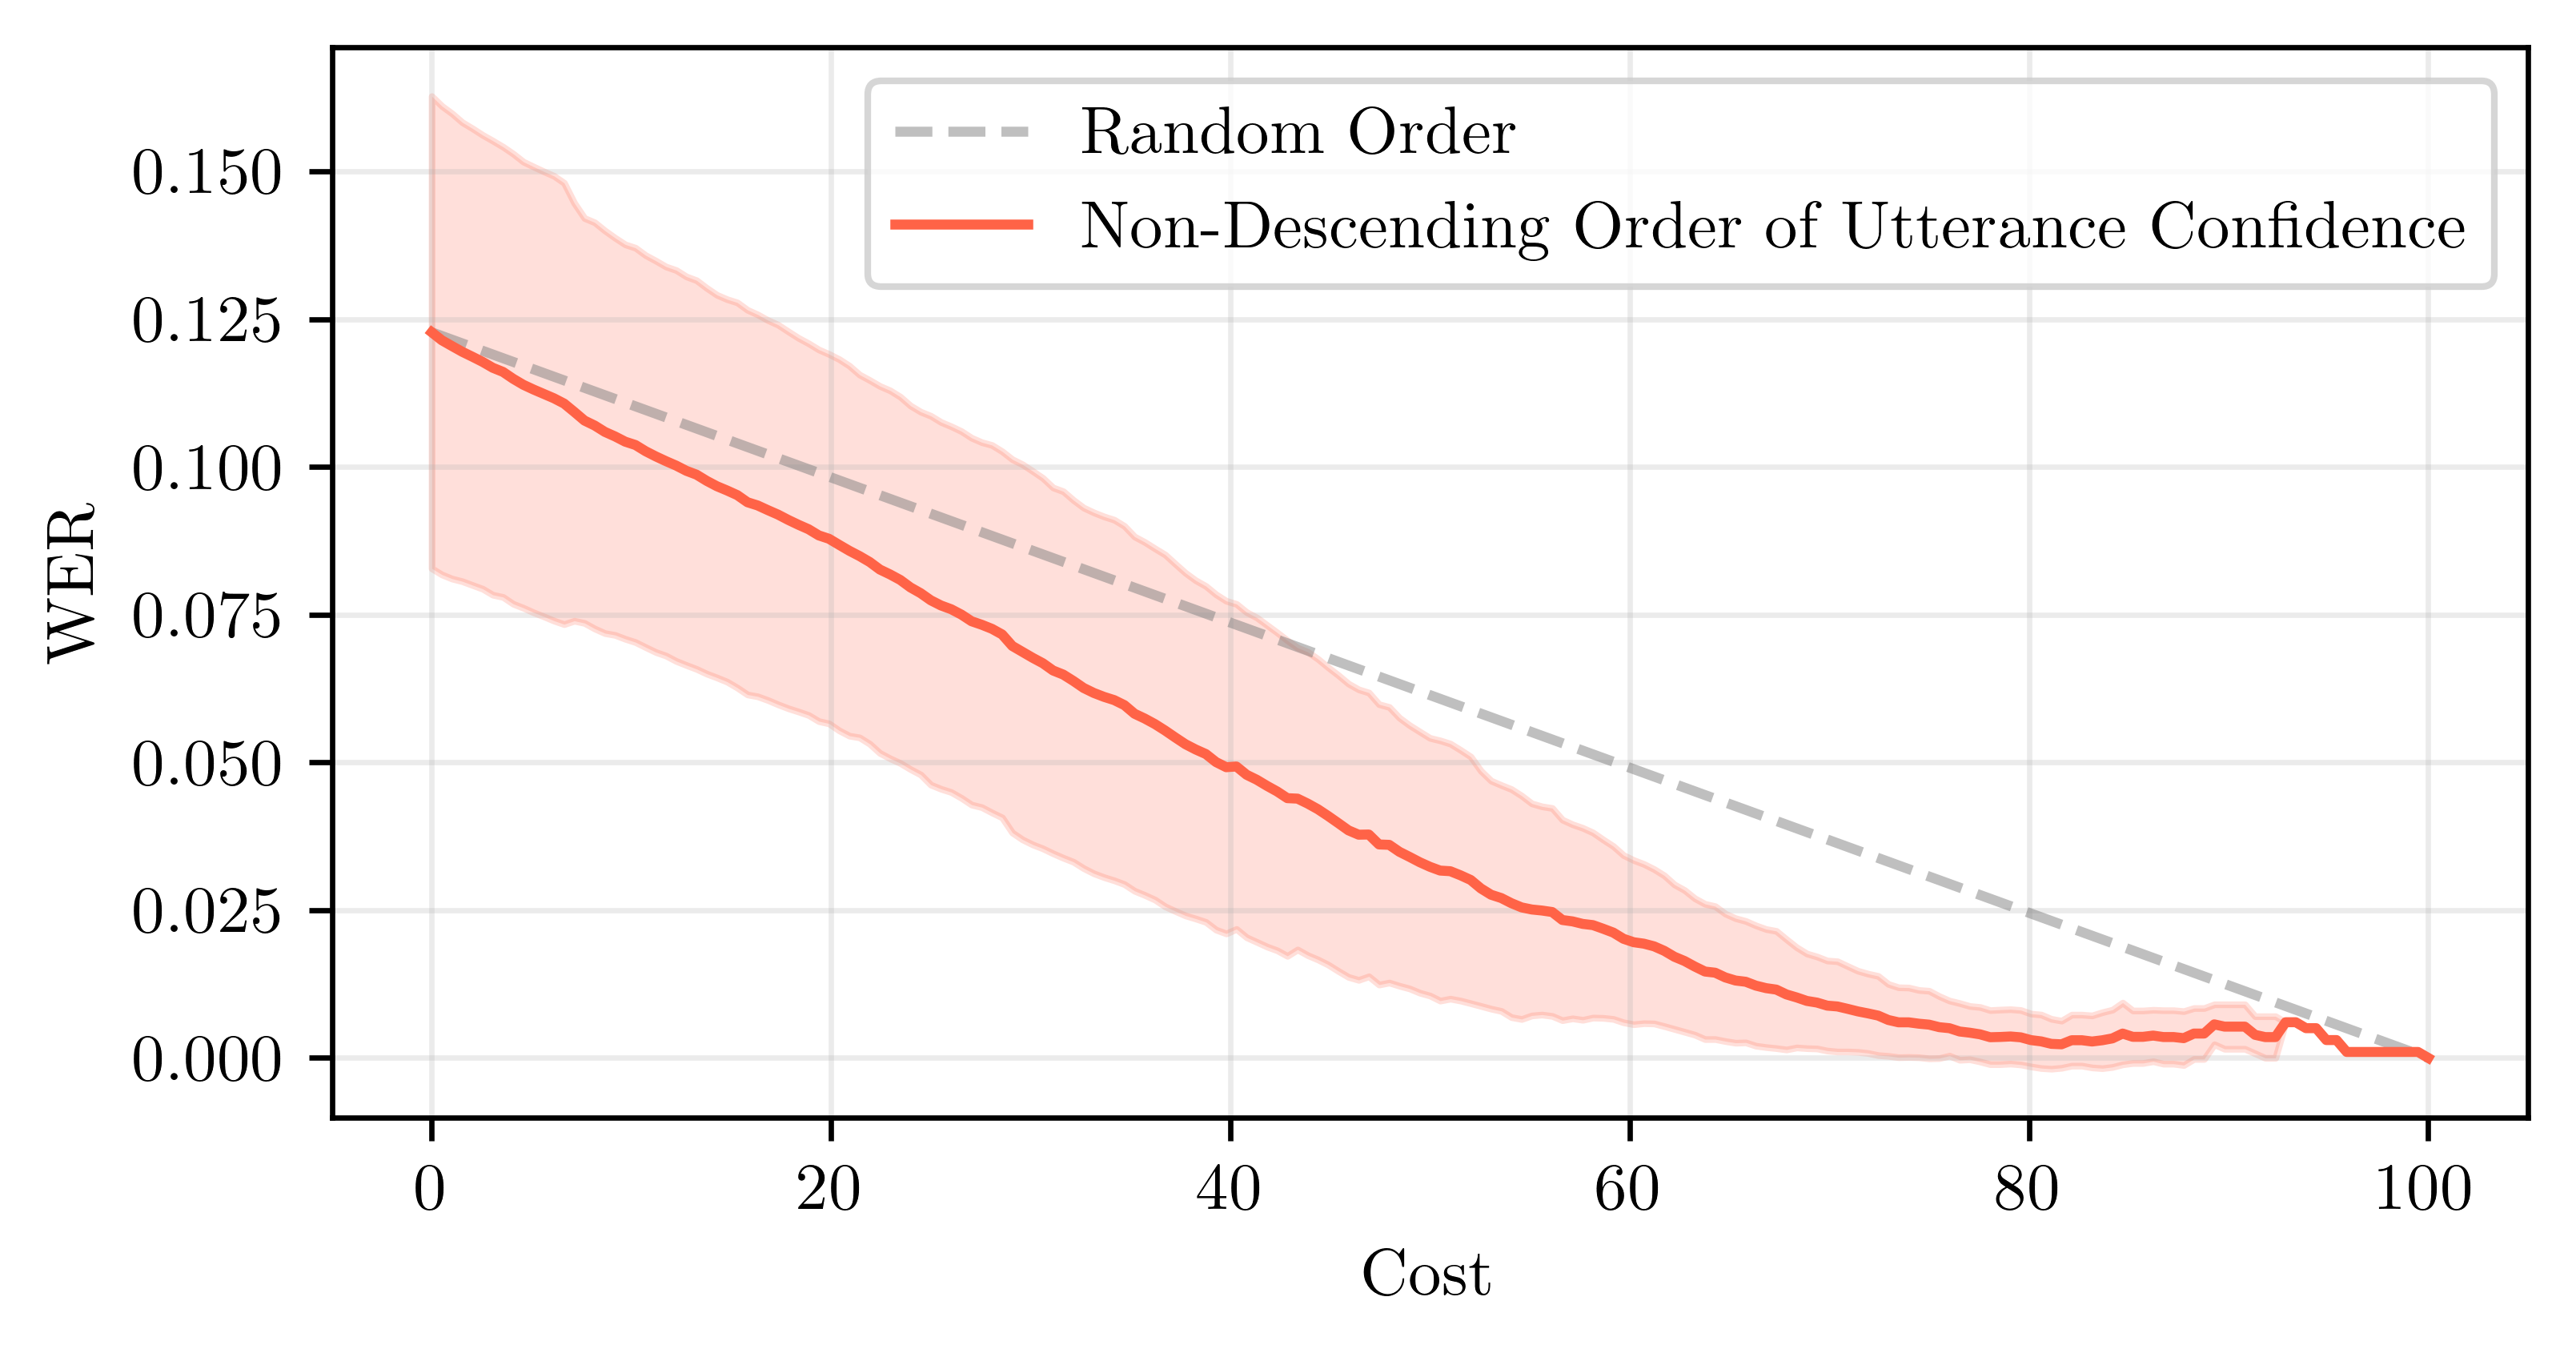
\includegraphics[width=\textwidth]{figures/average-uttconf.png}
 \centering
\end{figure}
\begin{figure}[p]
 \caption{Comparing per-conversation average performance of confidence and \texttt{avg\_logprob}}
 \label{fig:compare-avg-uttconf-vs-lprob}
 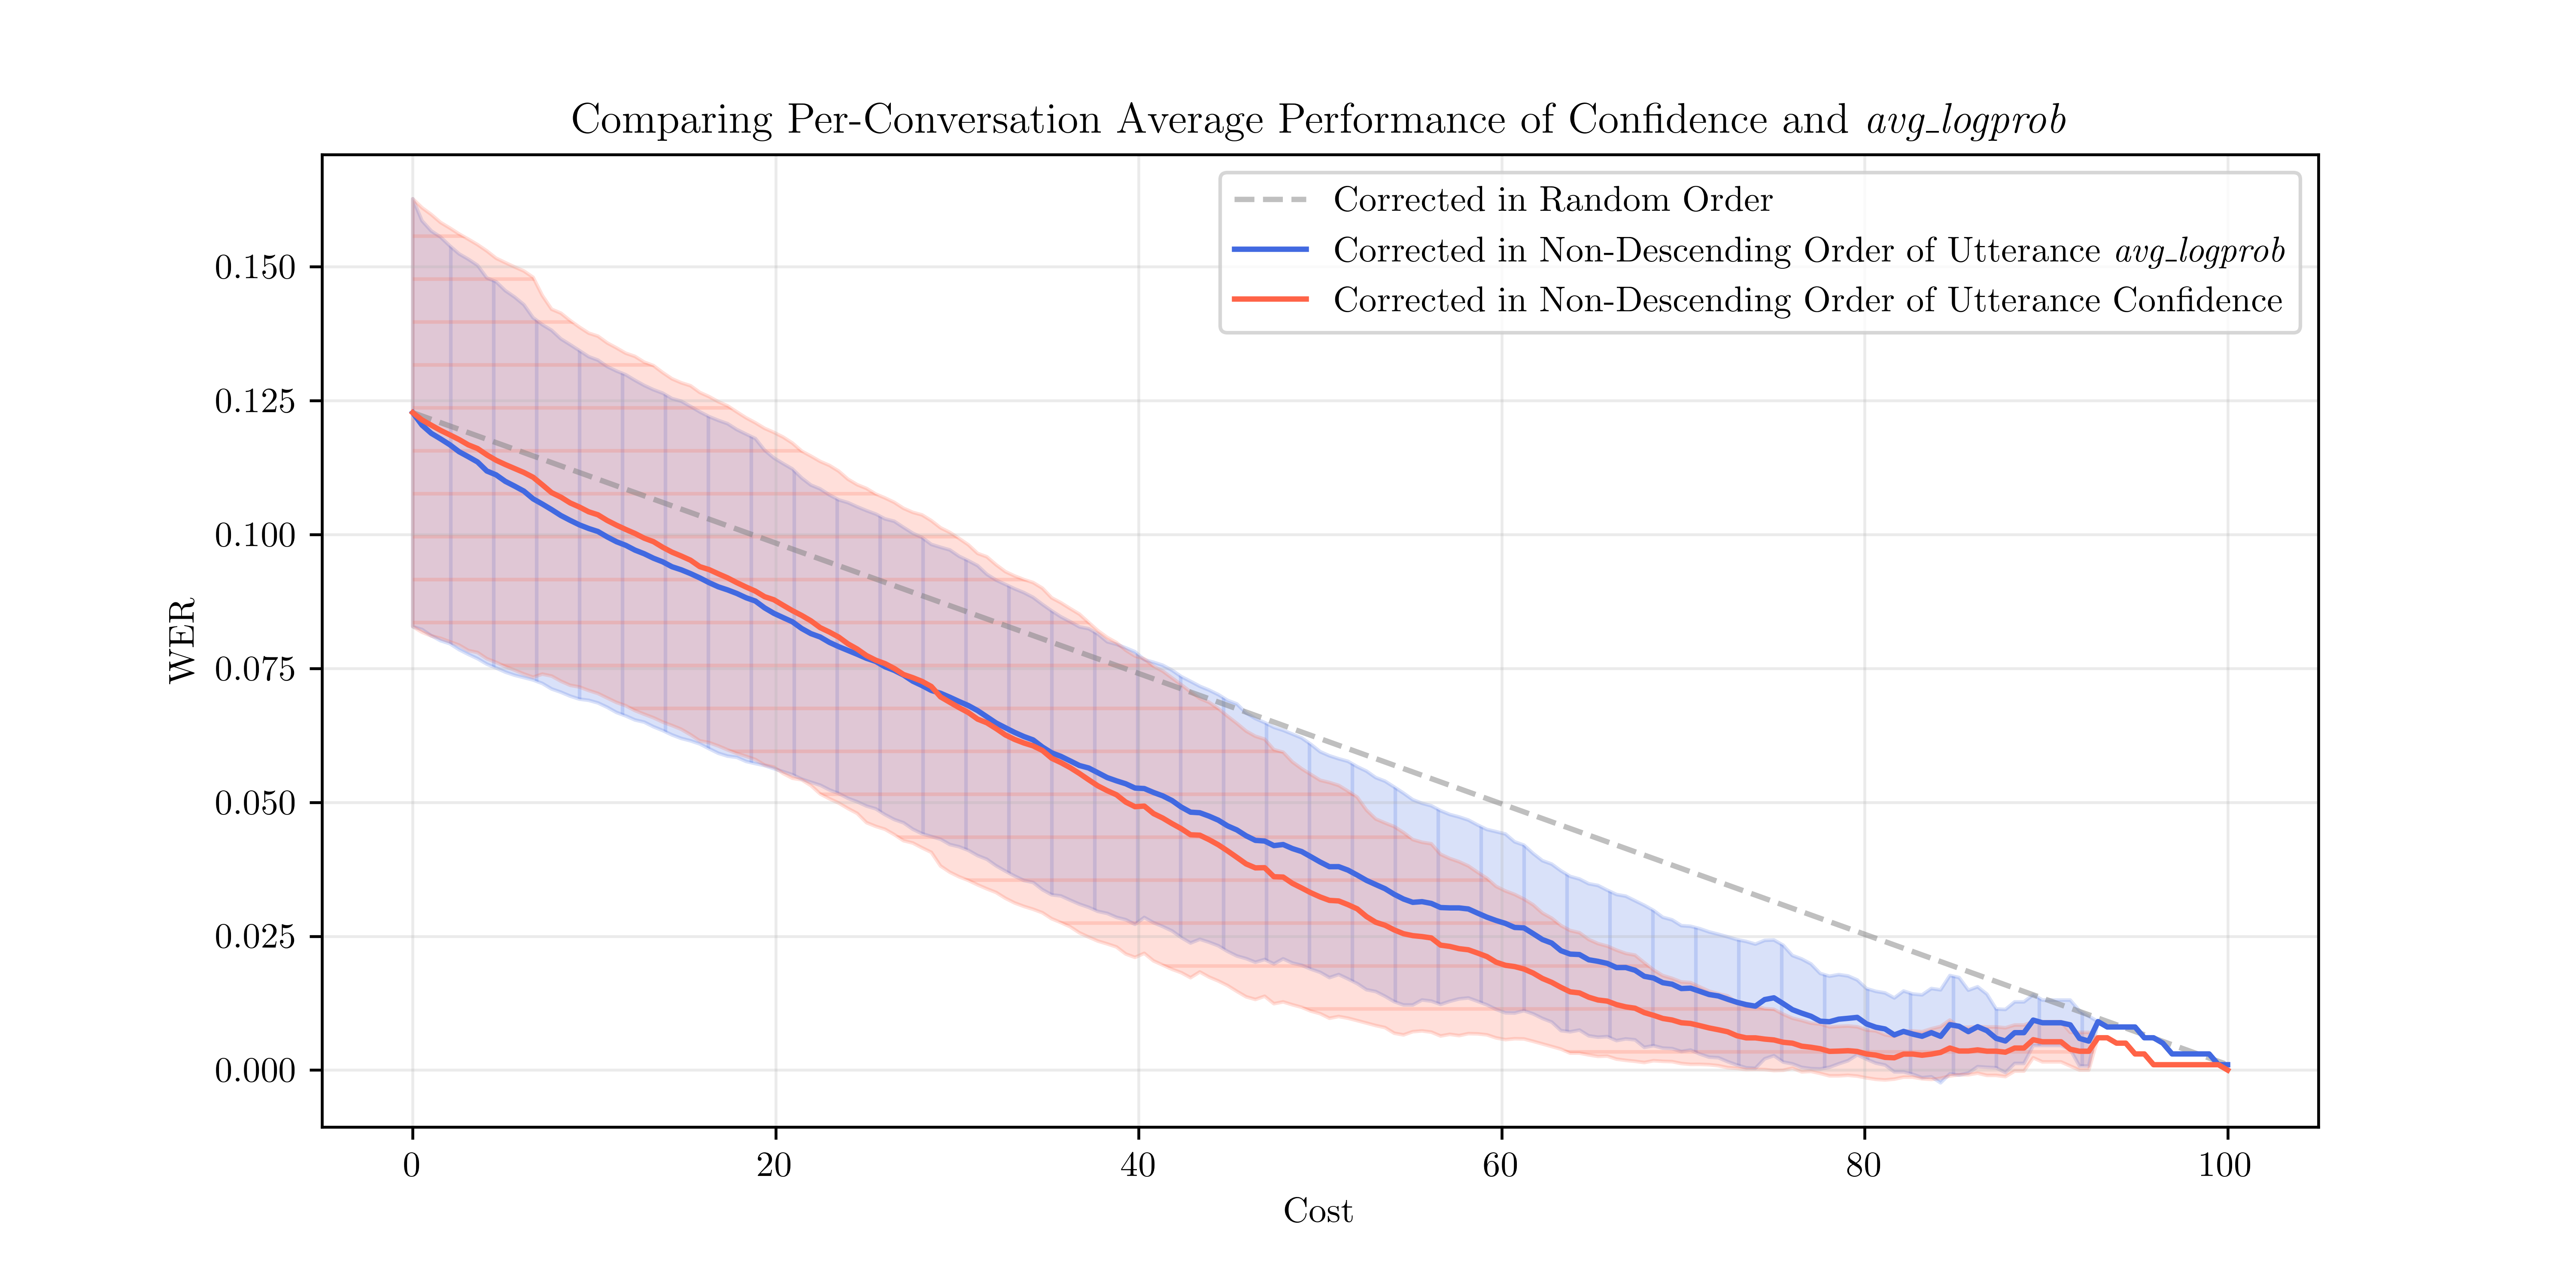
\includegraphics[width=\textwidth]{figures/compare-avg-uttconf-vs-lprob.png}
 \centering
\end{figure}
\begin{figure}[p]
 \caption{Comparing whole-corpus performance of confidence and \texttt{avg\_logprob}}
 \label{fig:corpus-avg-lprob-uttconf}
 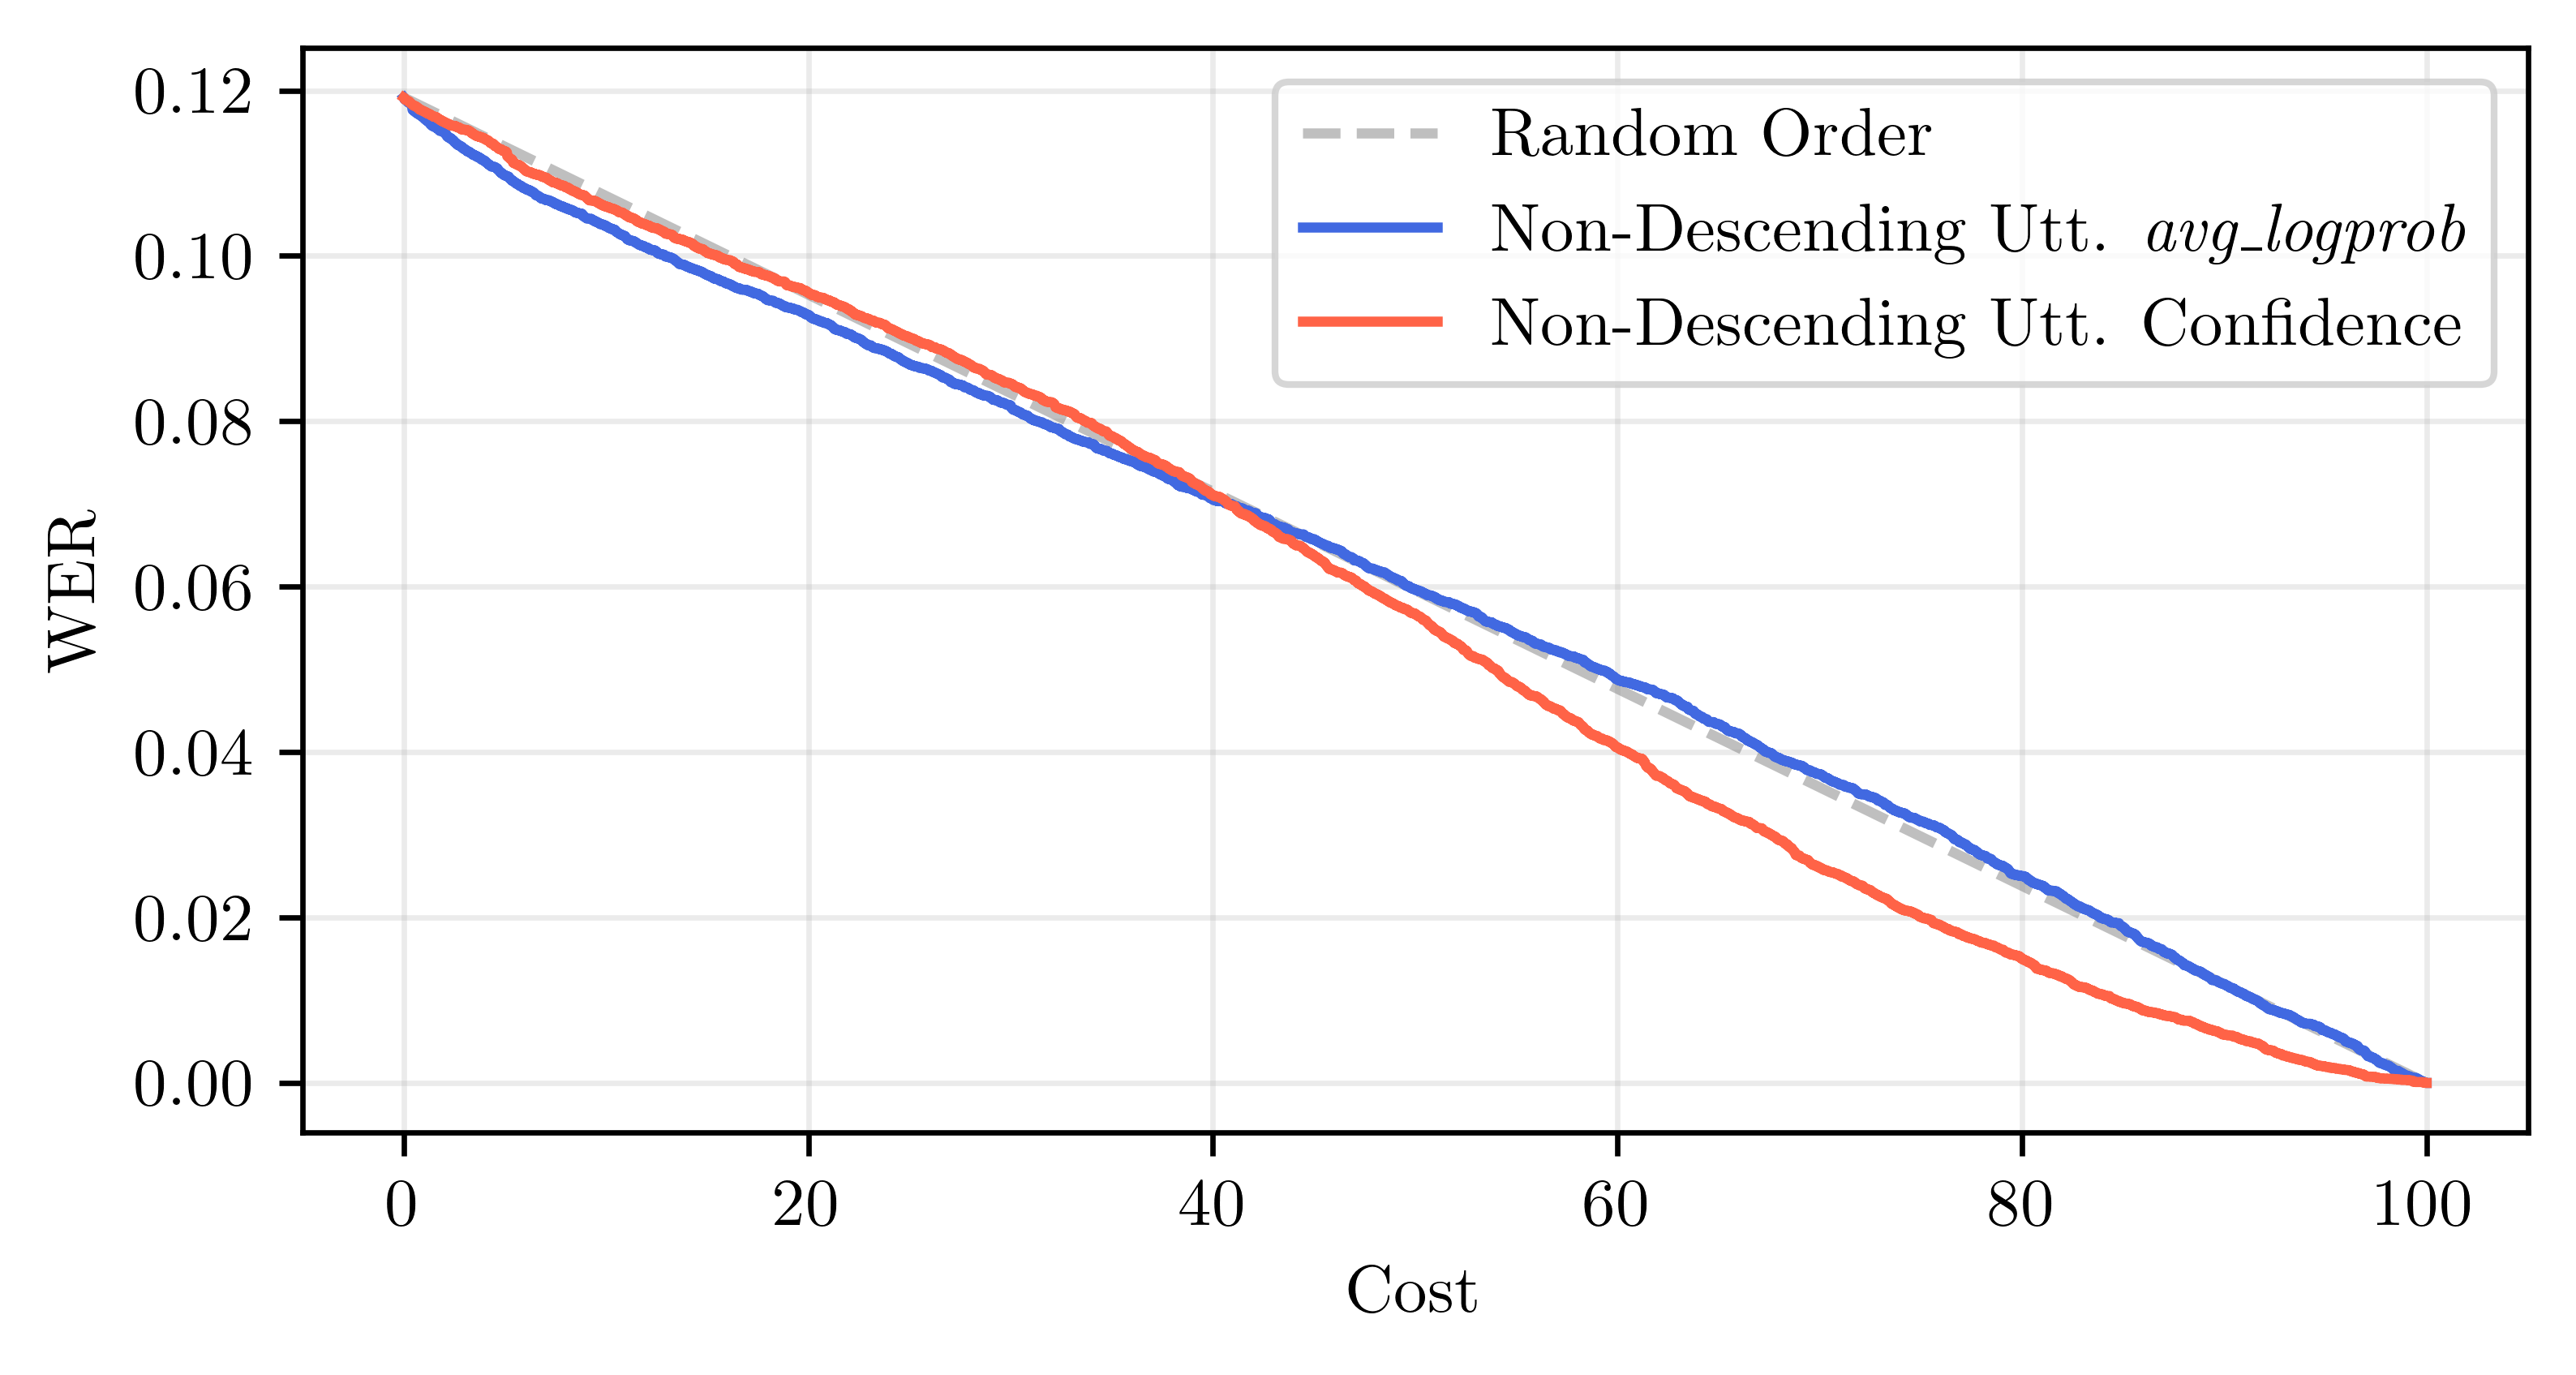
\includegraphics[width=\textwidth]{figures/corpus-avg-lprob-uttconf.png}
 \centering
\end{figure}

\clearpage
\subsection{Per-conversation average results using word-confidence}\label{subsec:avg-word-conf}

\begin{figure}[h!]
 \caption{Ordered by non-descending utterance-minimum word-confidence}
 \label{fig:word-conf-comparison-plot1}
 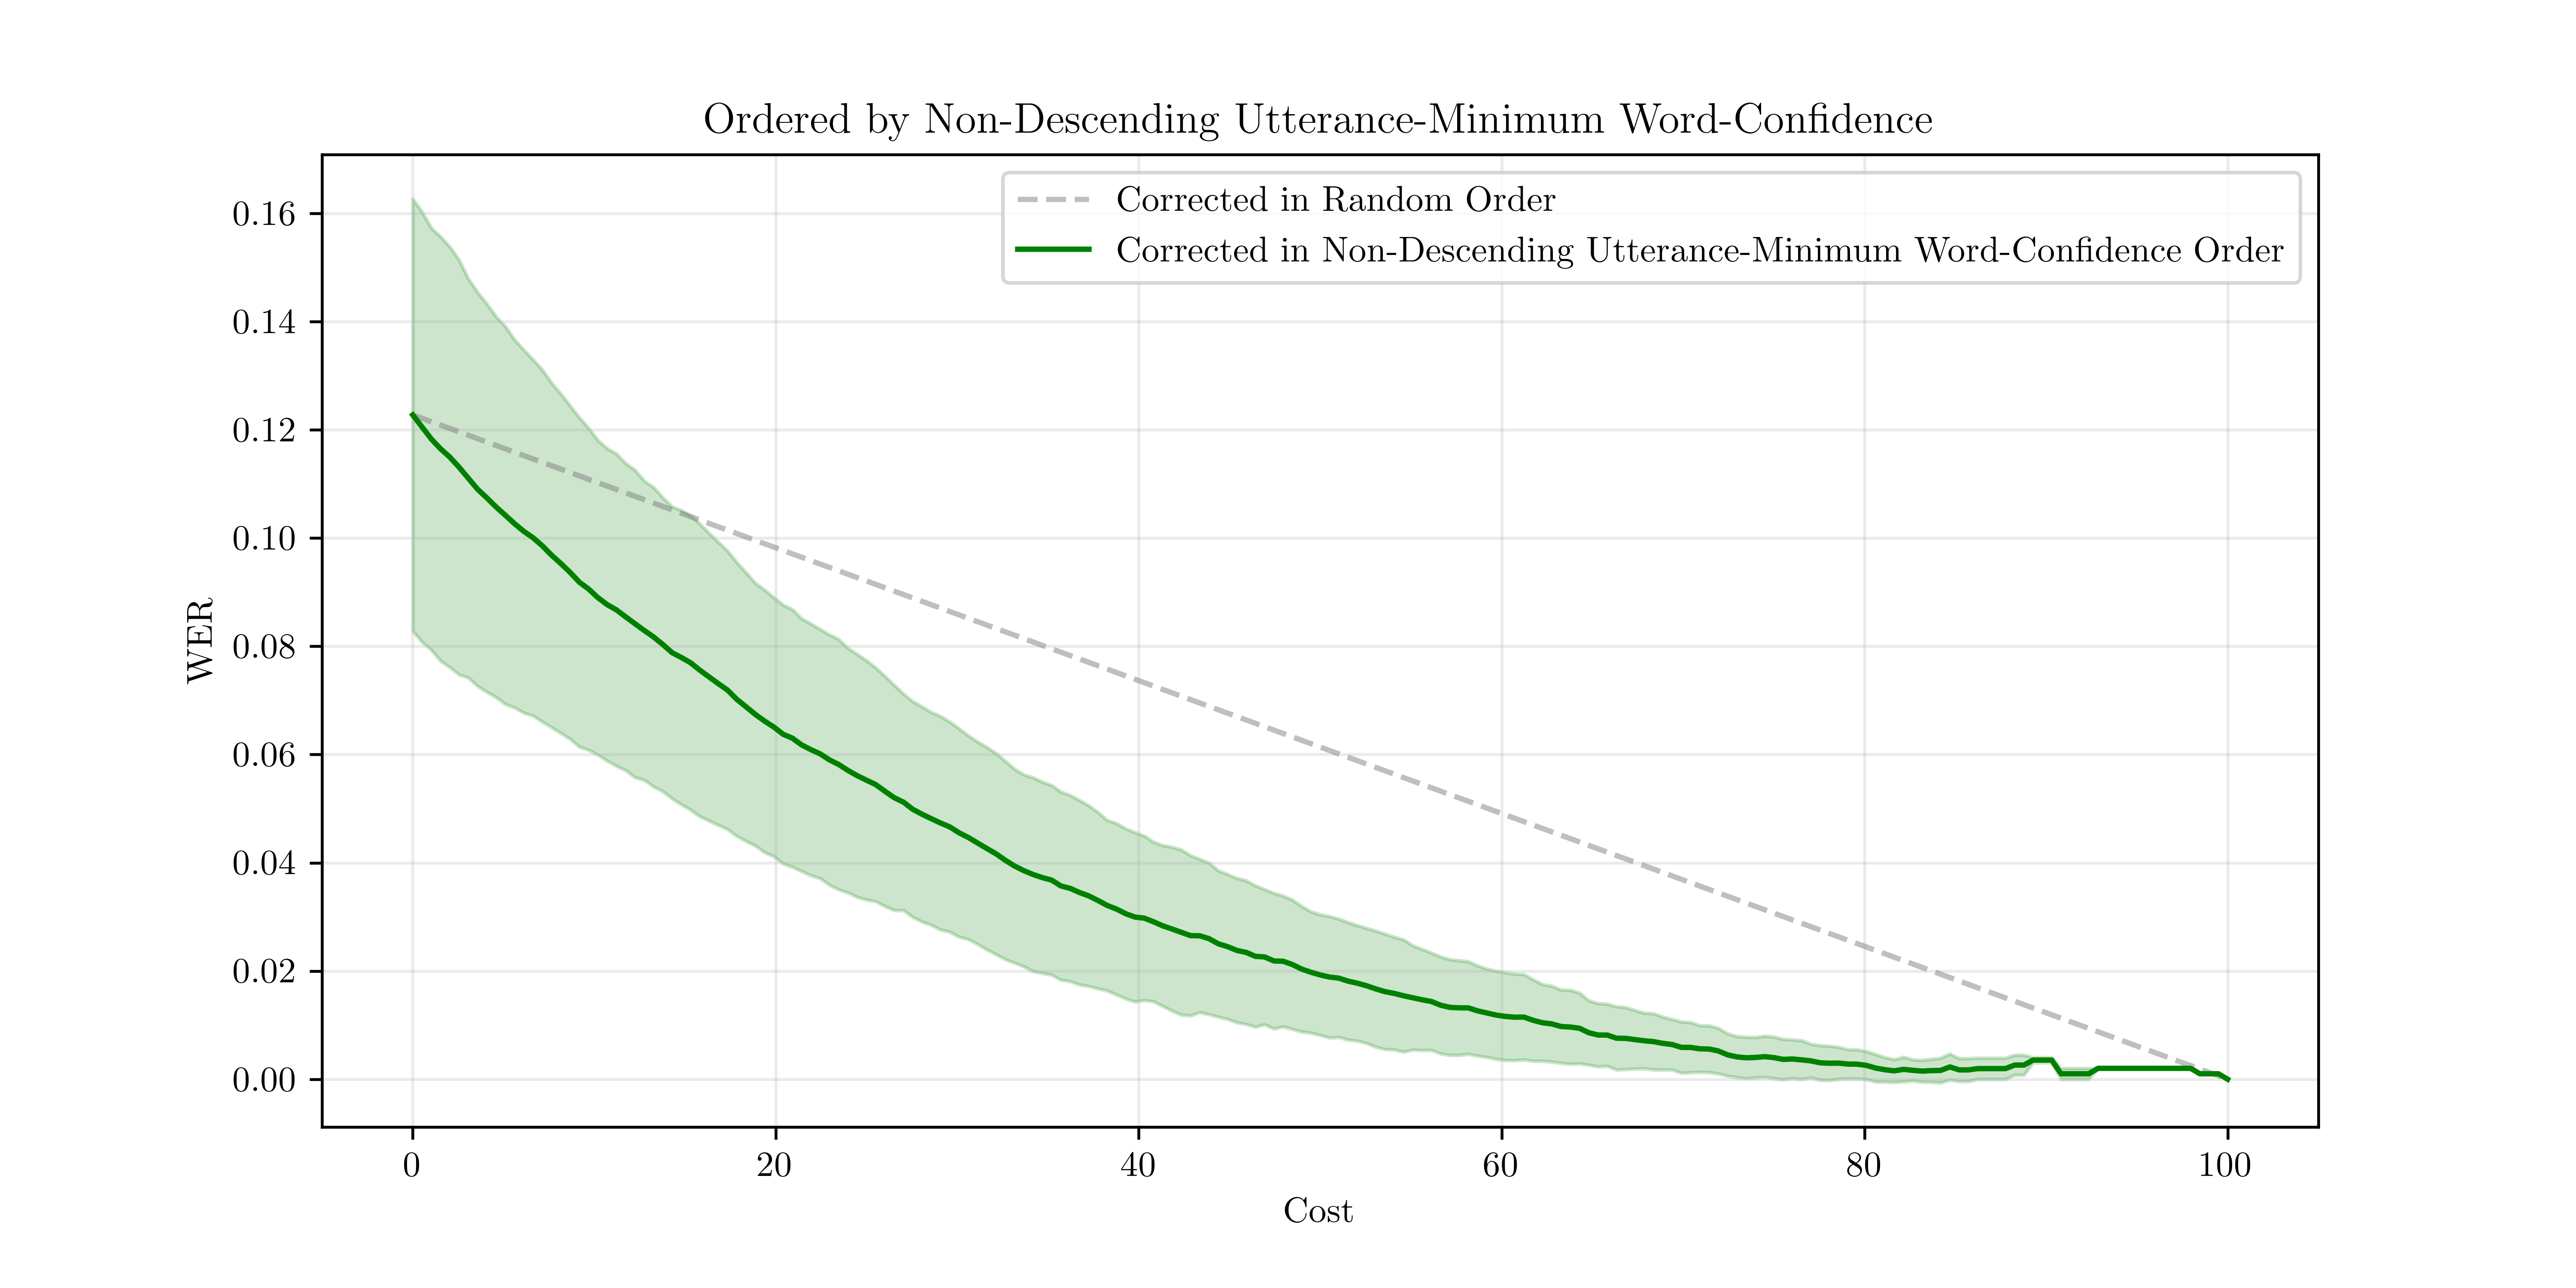
\includegraphics[width=\textwidth]{figures/word-conf-comparison-plot1.png}
 \centering
\end{figure}
\begin{figure}[h!]
 \caption{Ordered by non-ascending utterance-minimum word-confidence}
 \label{fig:word-conf-comparison-plot2}
 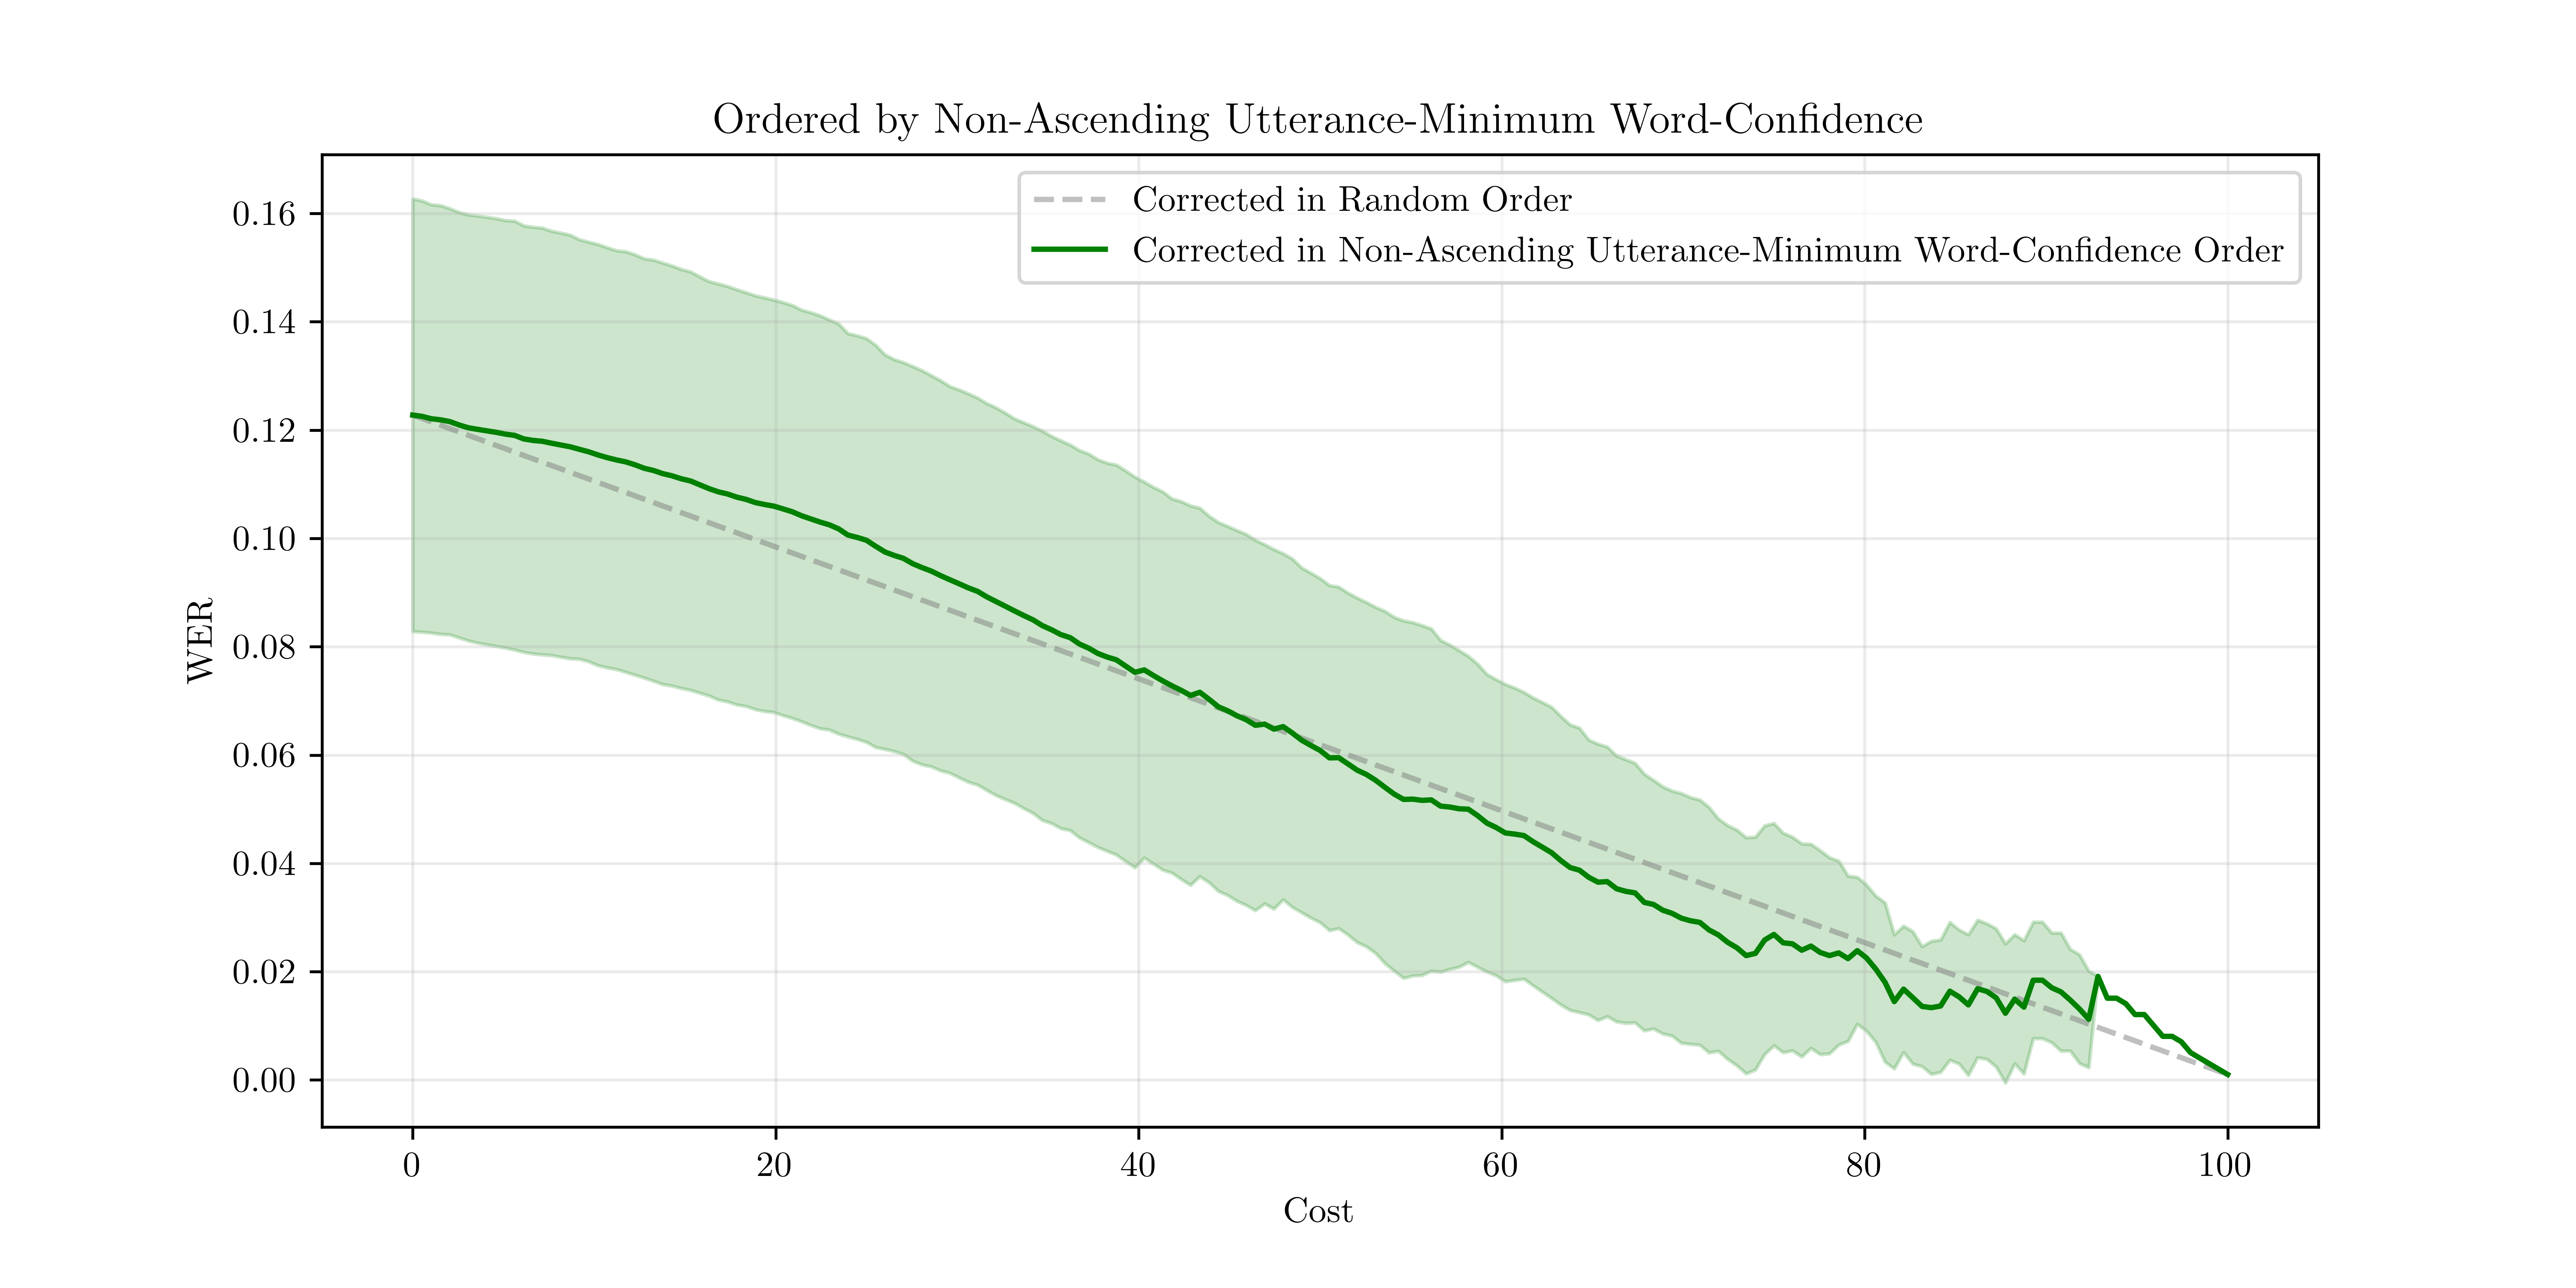
\includegraphics[width=\textwidth]{figures/word-conf-comparison-plot2.png}
 \centering
\end{figure}
\begin{figure}[p]
 \caption{Ordered by non-descending utterance-maximum word-confidence}
 \label{fig:word-conf-comparison-plot3}
 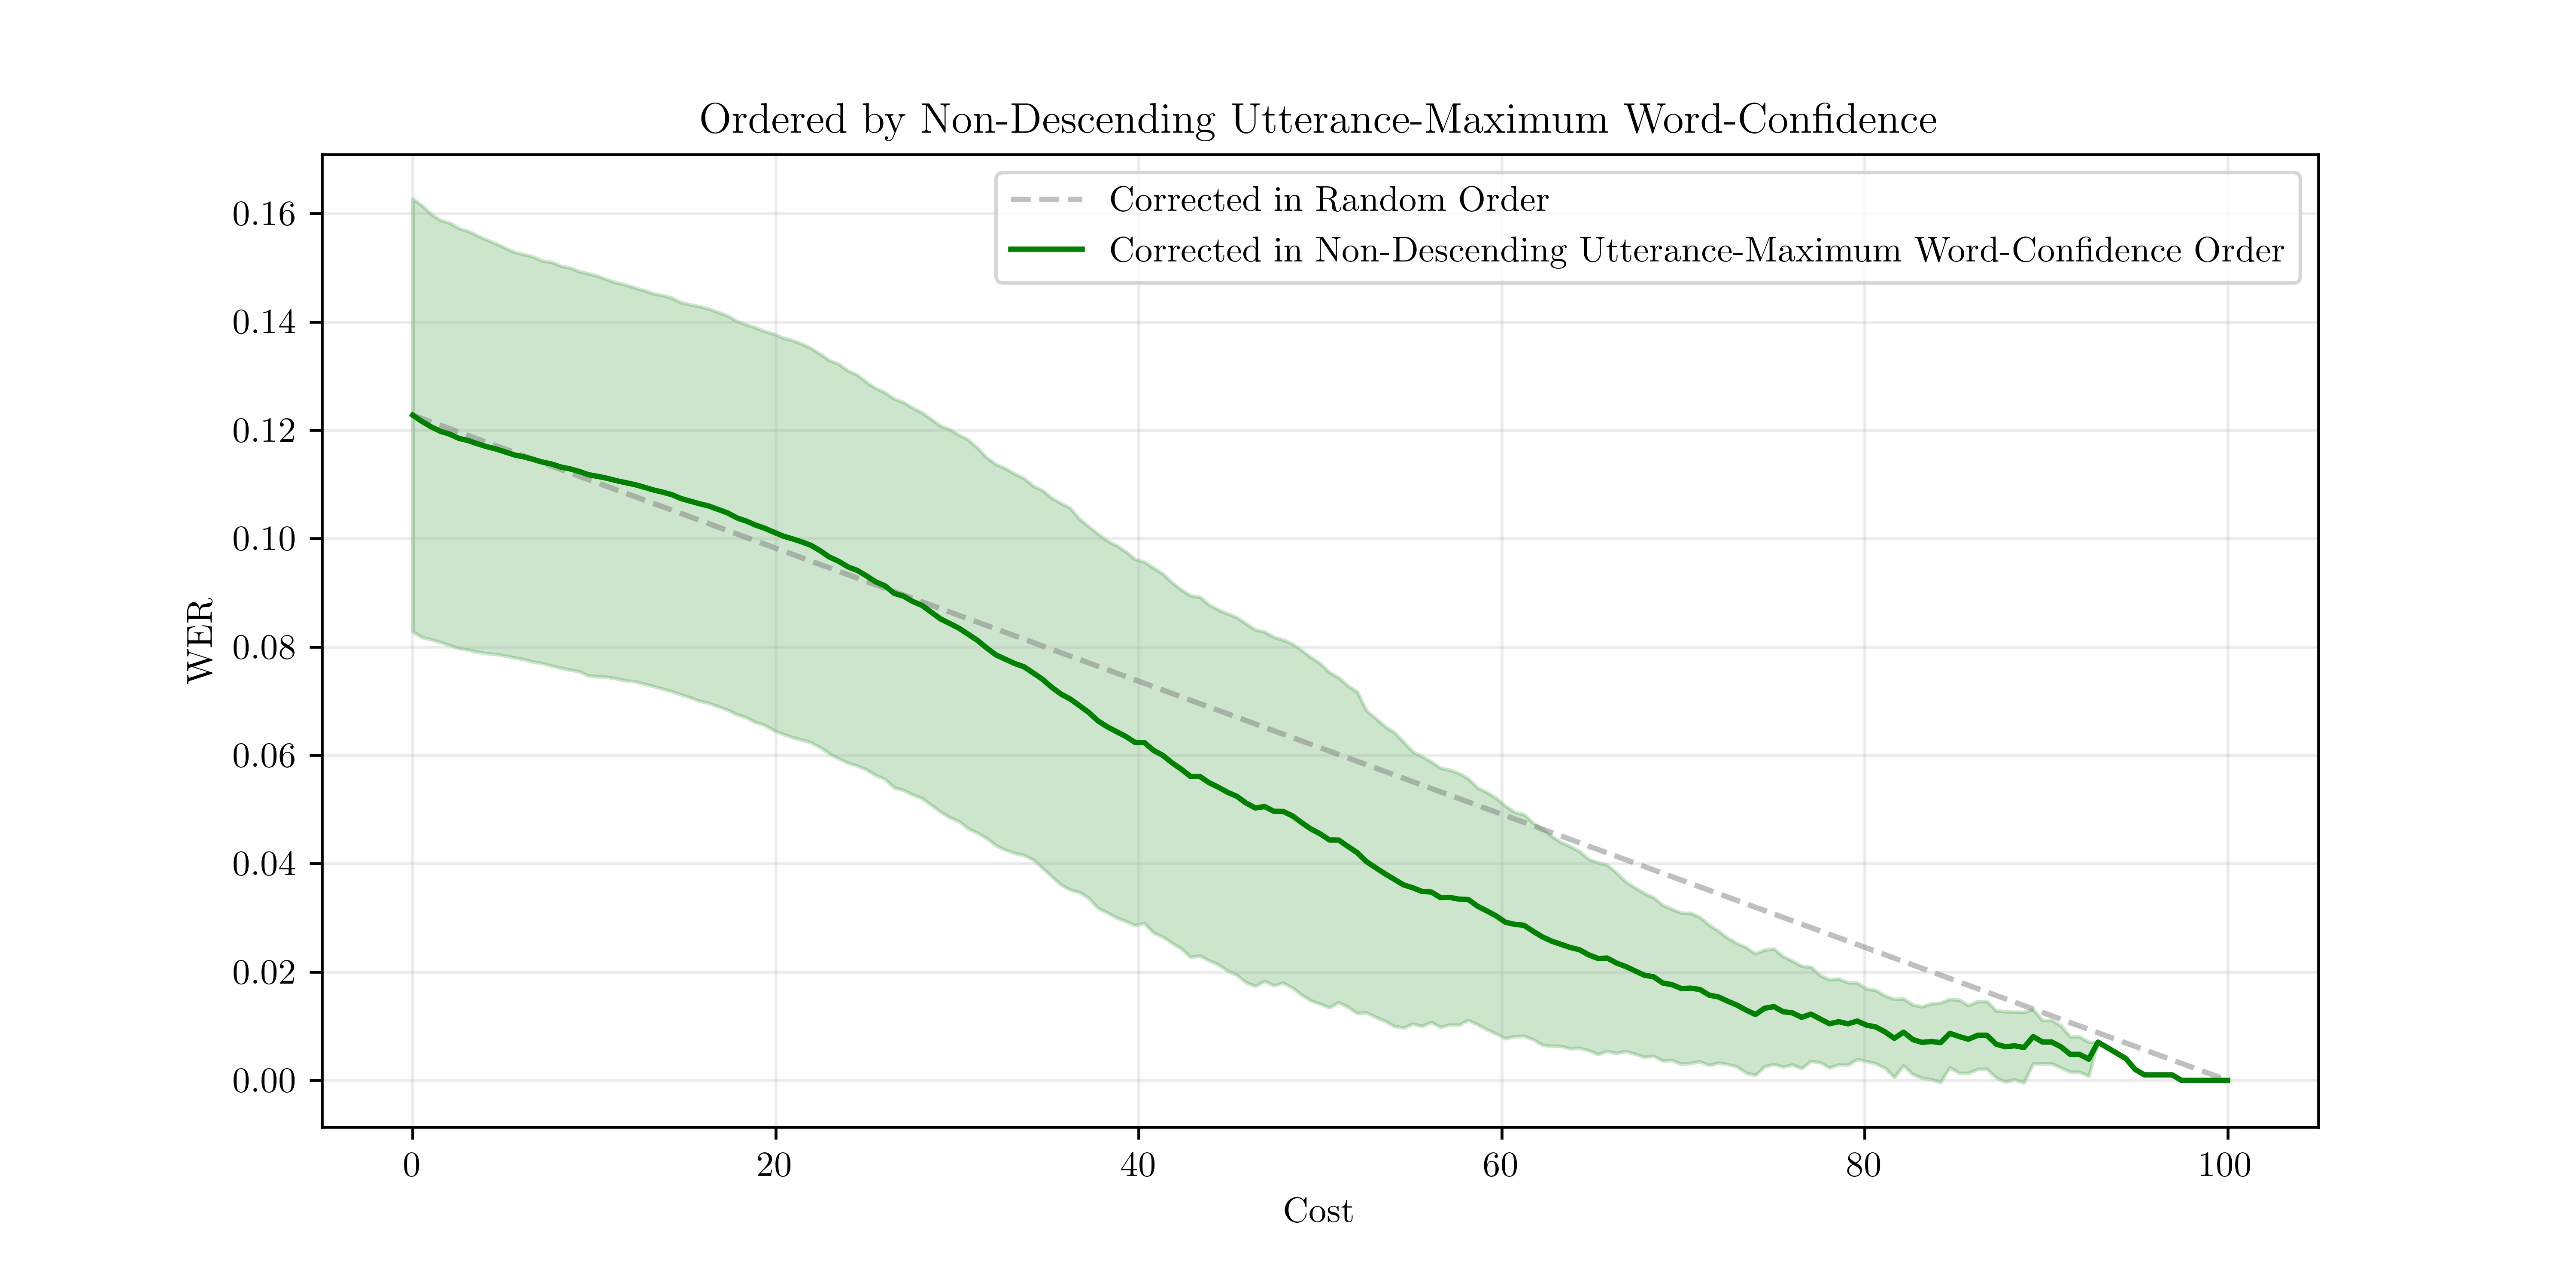
\includegraphics[width=\textwidth]{figures/word-conf-comparison-plot3.png}
 \centering
\end{figure}
\begin{figure}[p]
 \caption{Ordered by non-ascending utterance-maximum word-confidence}
 \label{fig:word-conf-comparison-plot4}
 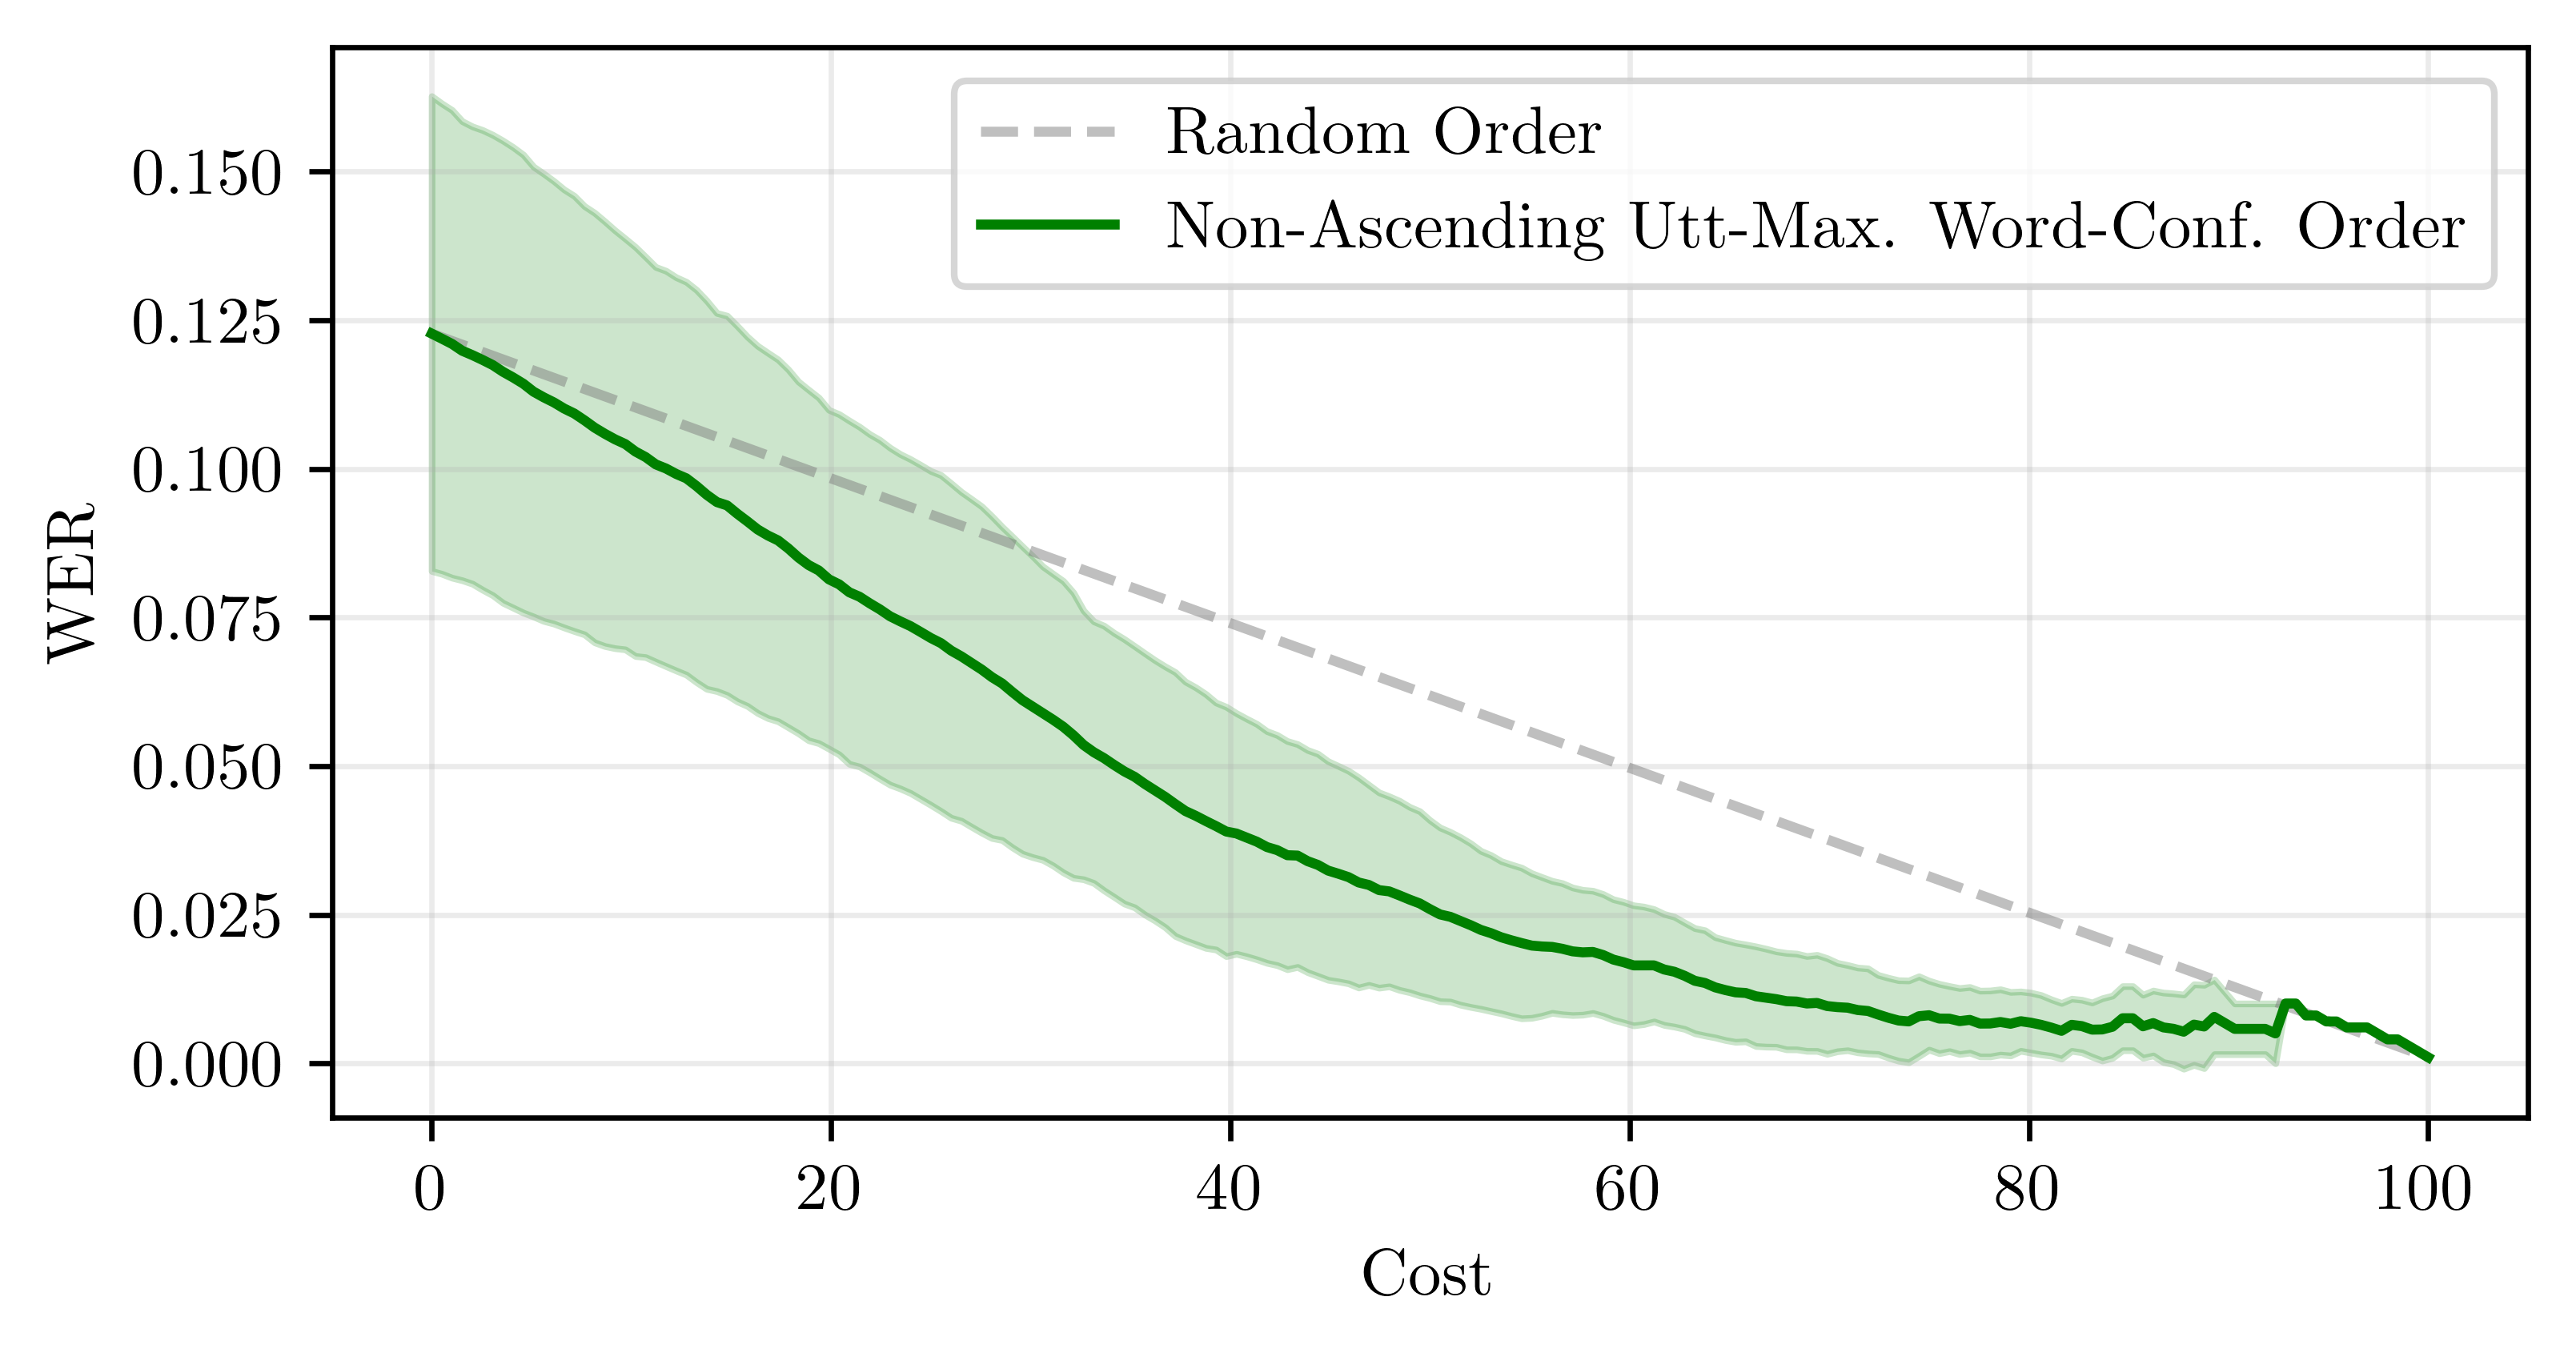
\includegraphics[width=\textwidth]{figures/word-conf-comparison-plot4.png}
 \centering
\end{figure}

\clearpage
\subsection{Corpus-wide comparisons with word-level confidence ordering}\label{subsec:comparing-all}

\begin{figure}[h!]
 \caption{Comparing whole-corpus evaluation performance with each word-confidence ordering}
 \label{fig:corpus-all-word-conf-measures}
 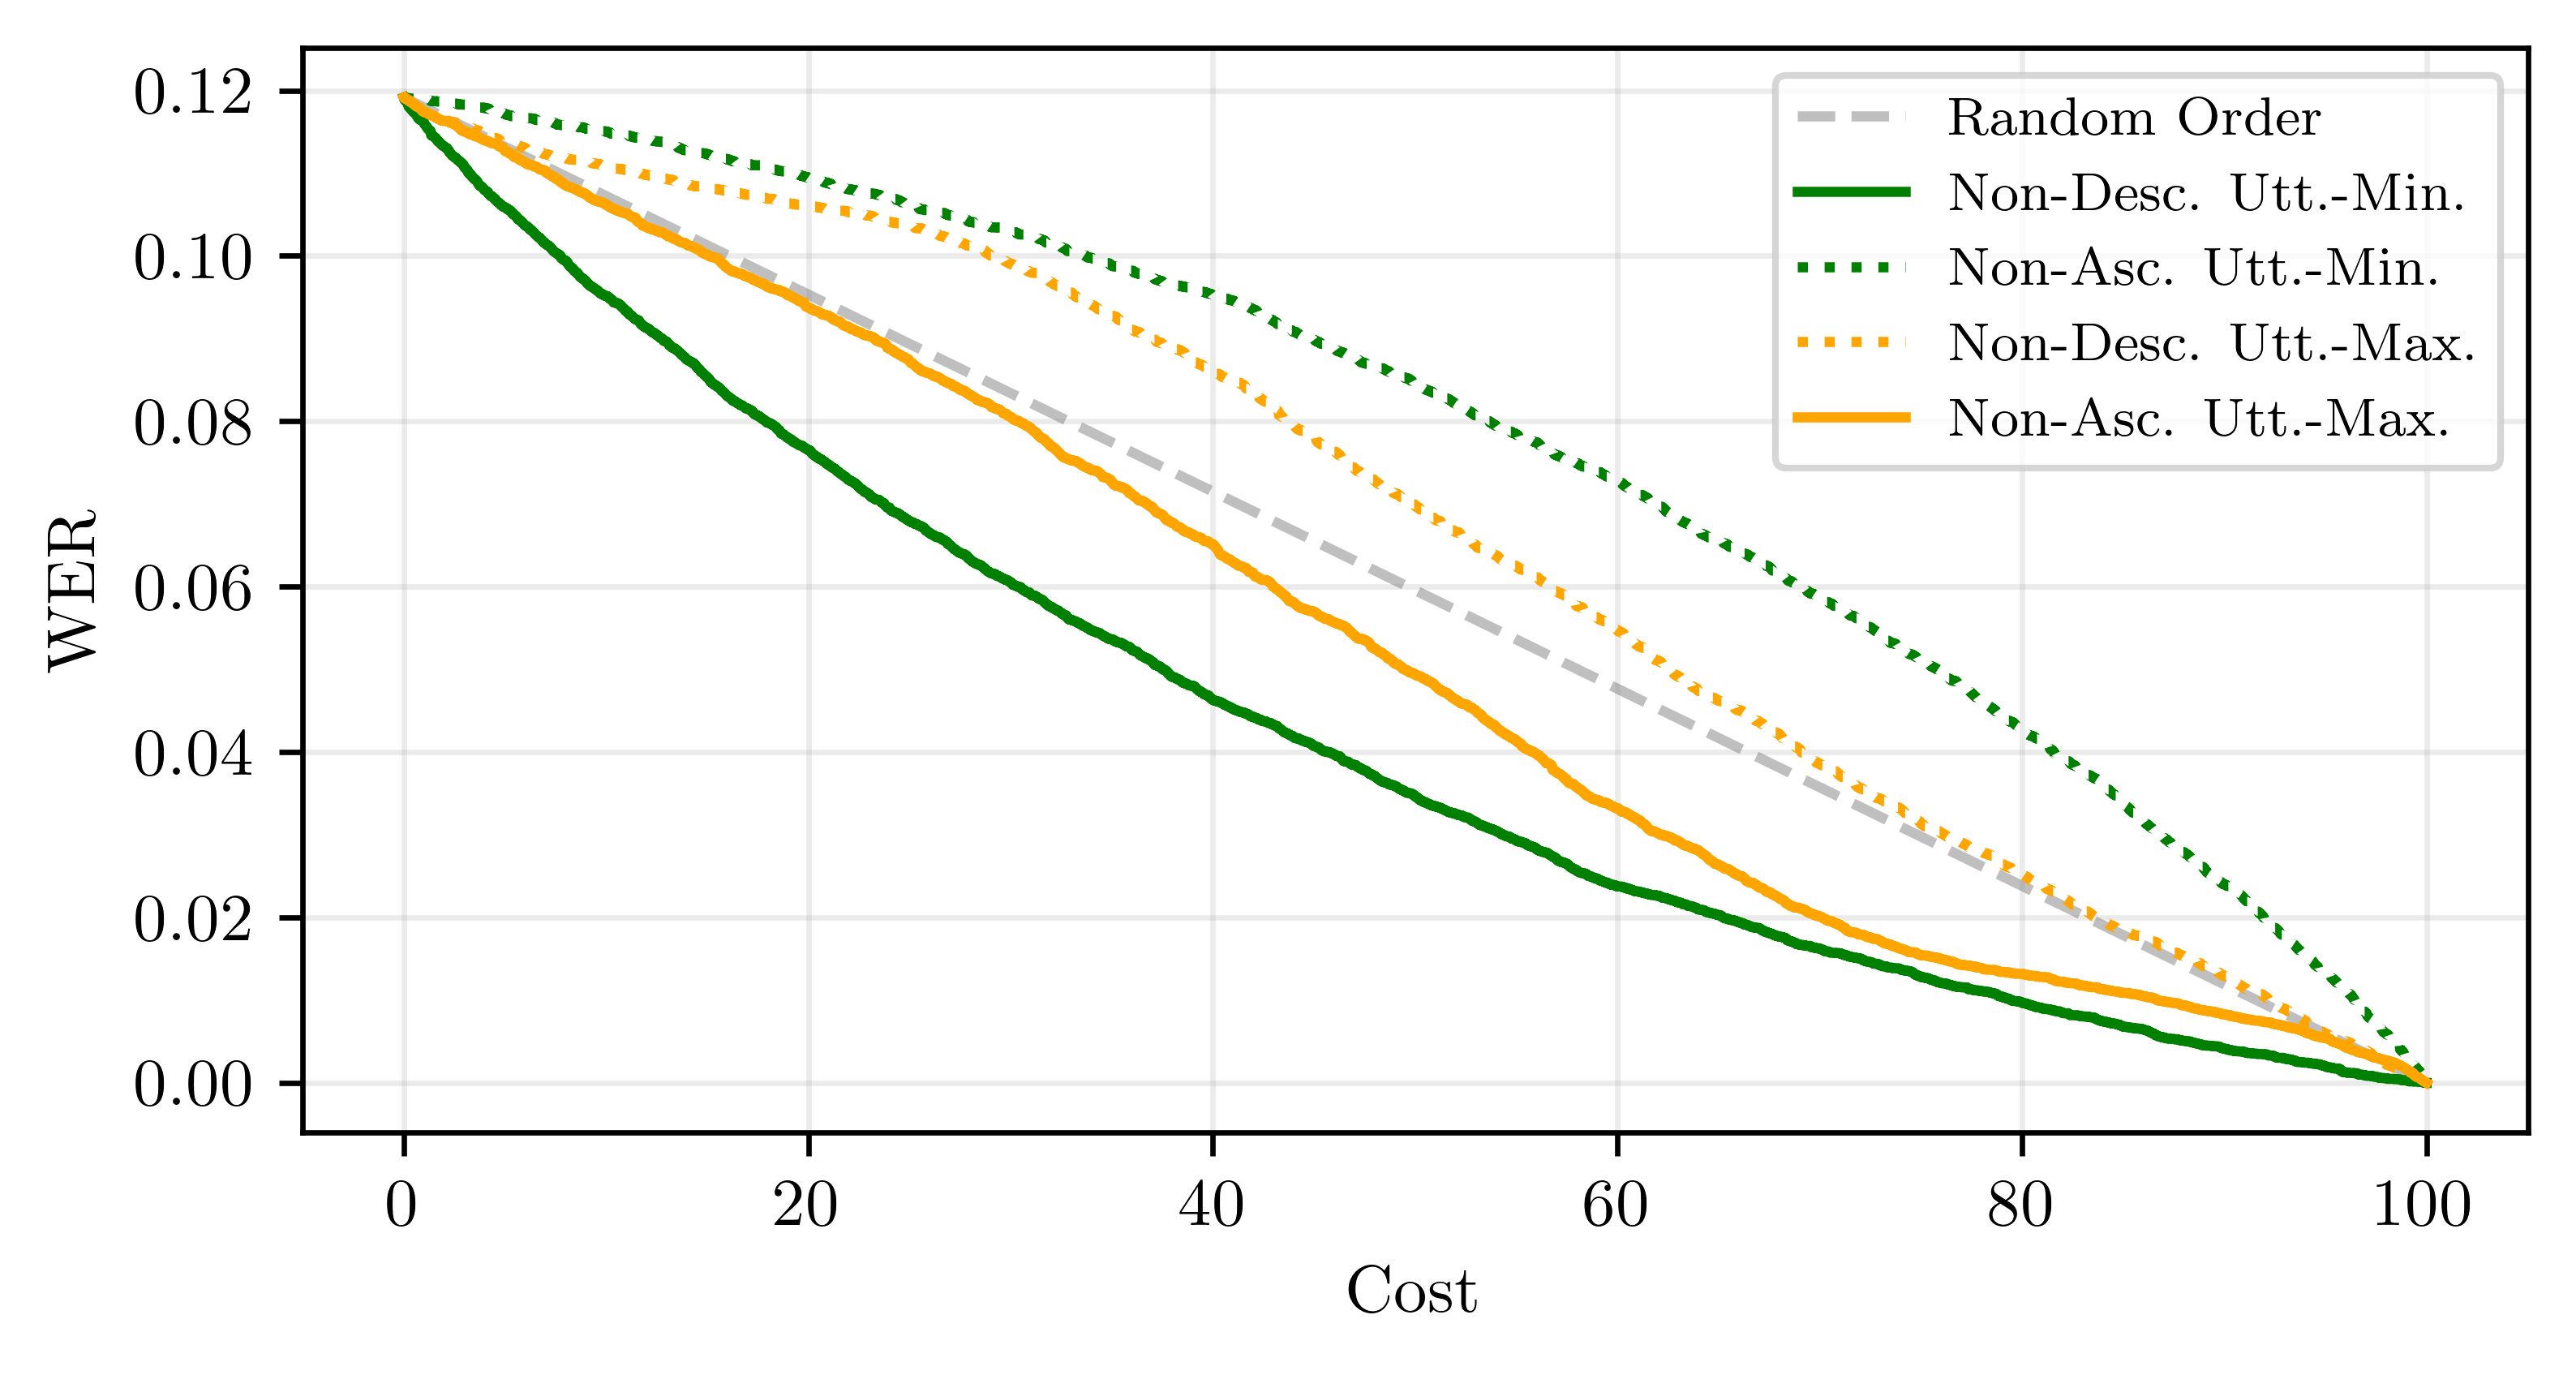
\includegraphics[width=\textwidth]{figures/corpus-all-word-conf-measures.png}
 \centering
\end{figure}
\begin{figure}[h!]
 \caption{Comparing whole-corpus evaluation performance with each ordering metric}
 \label{fig:corpus-allmeasures}
 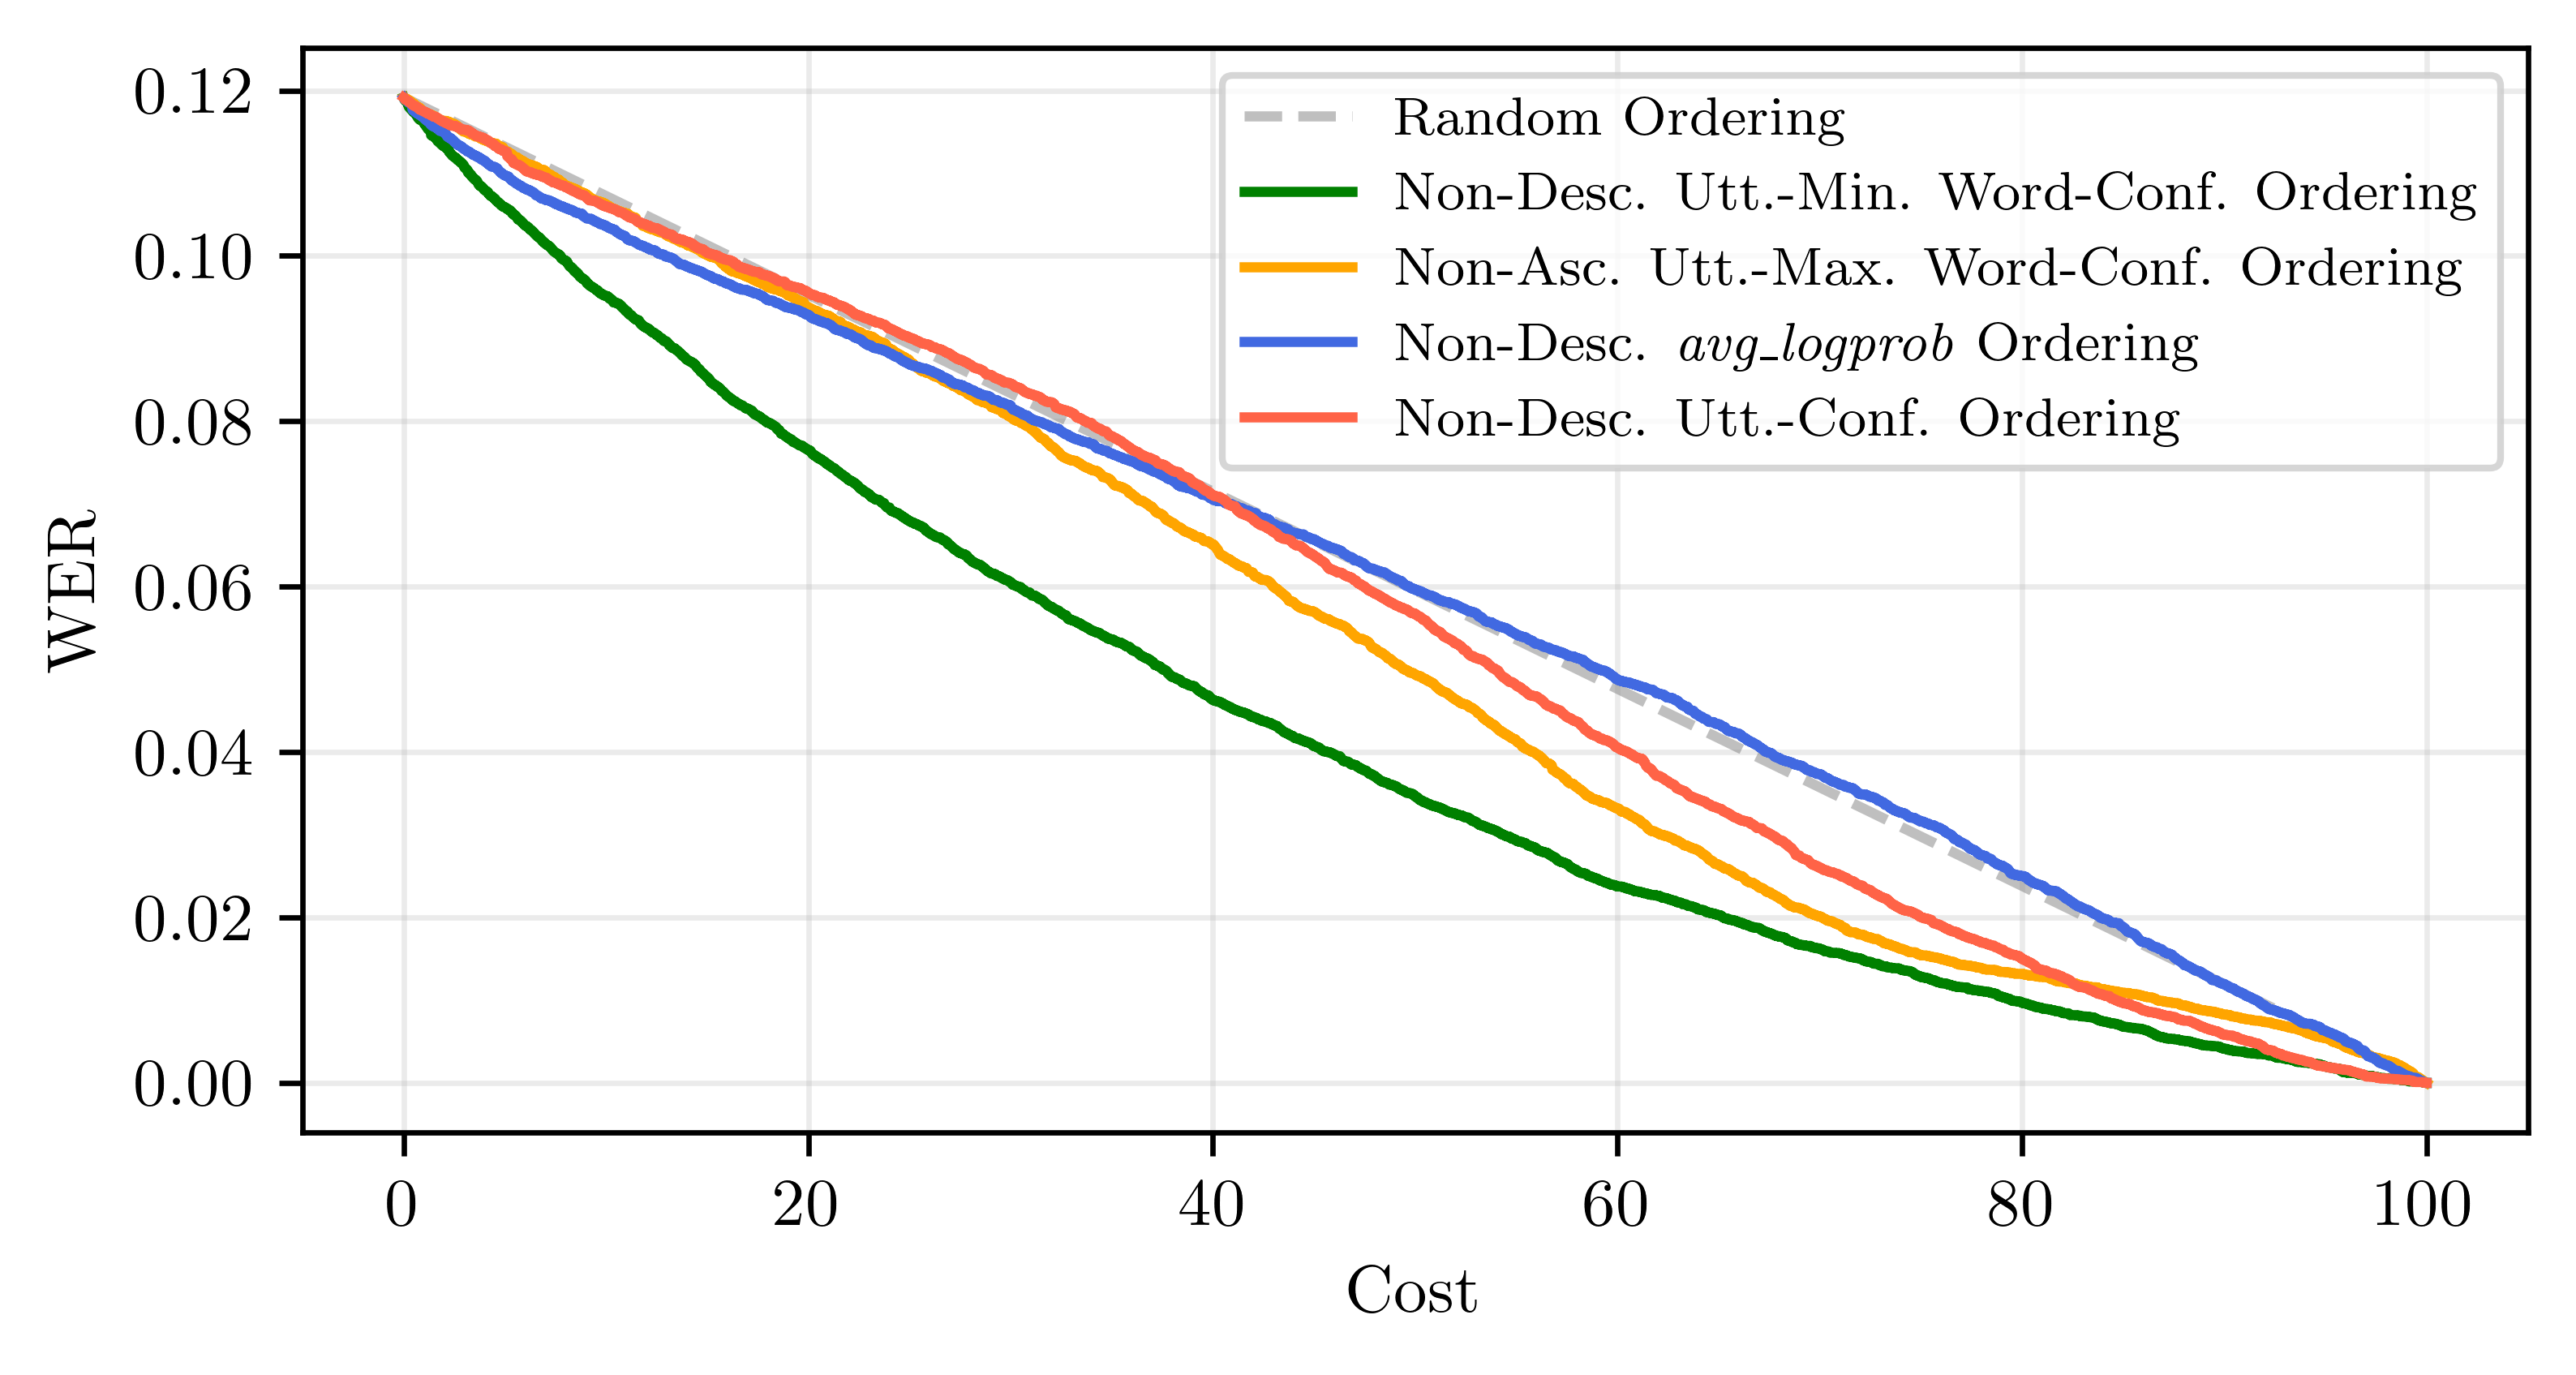
\includegraphics[width=\textwidth]{figures/corpus-allmeasures.png}
 \centering
\end{figure}

\clearpage
\subsection{Different word-level confidence scoring techniques}\label{subsec:more-techniques}

\begin{figure}[h!]
 \caption{Comparing whole-corpus evaluation performance with different word-level confidence metrics}
 \label{fig:range-ordering-vs-stddev-vs-min-wconf}
 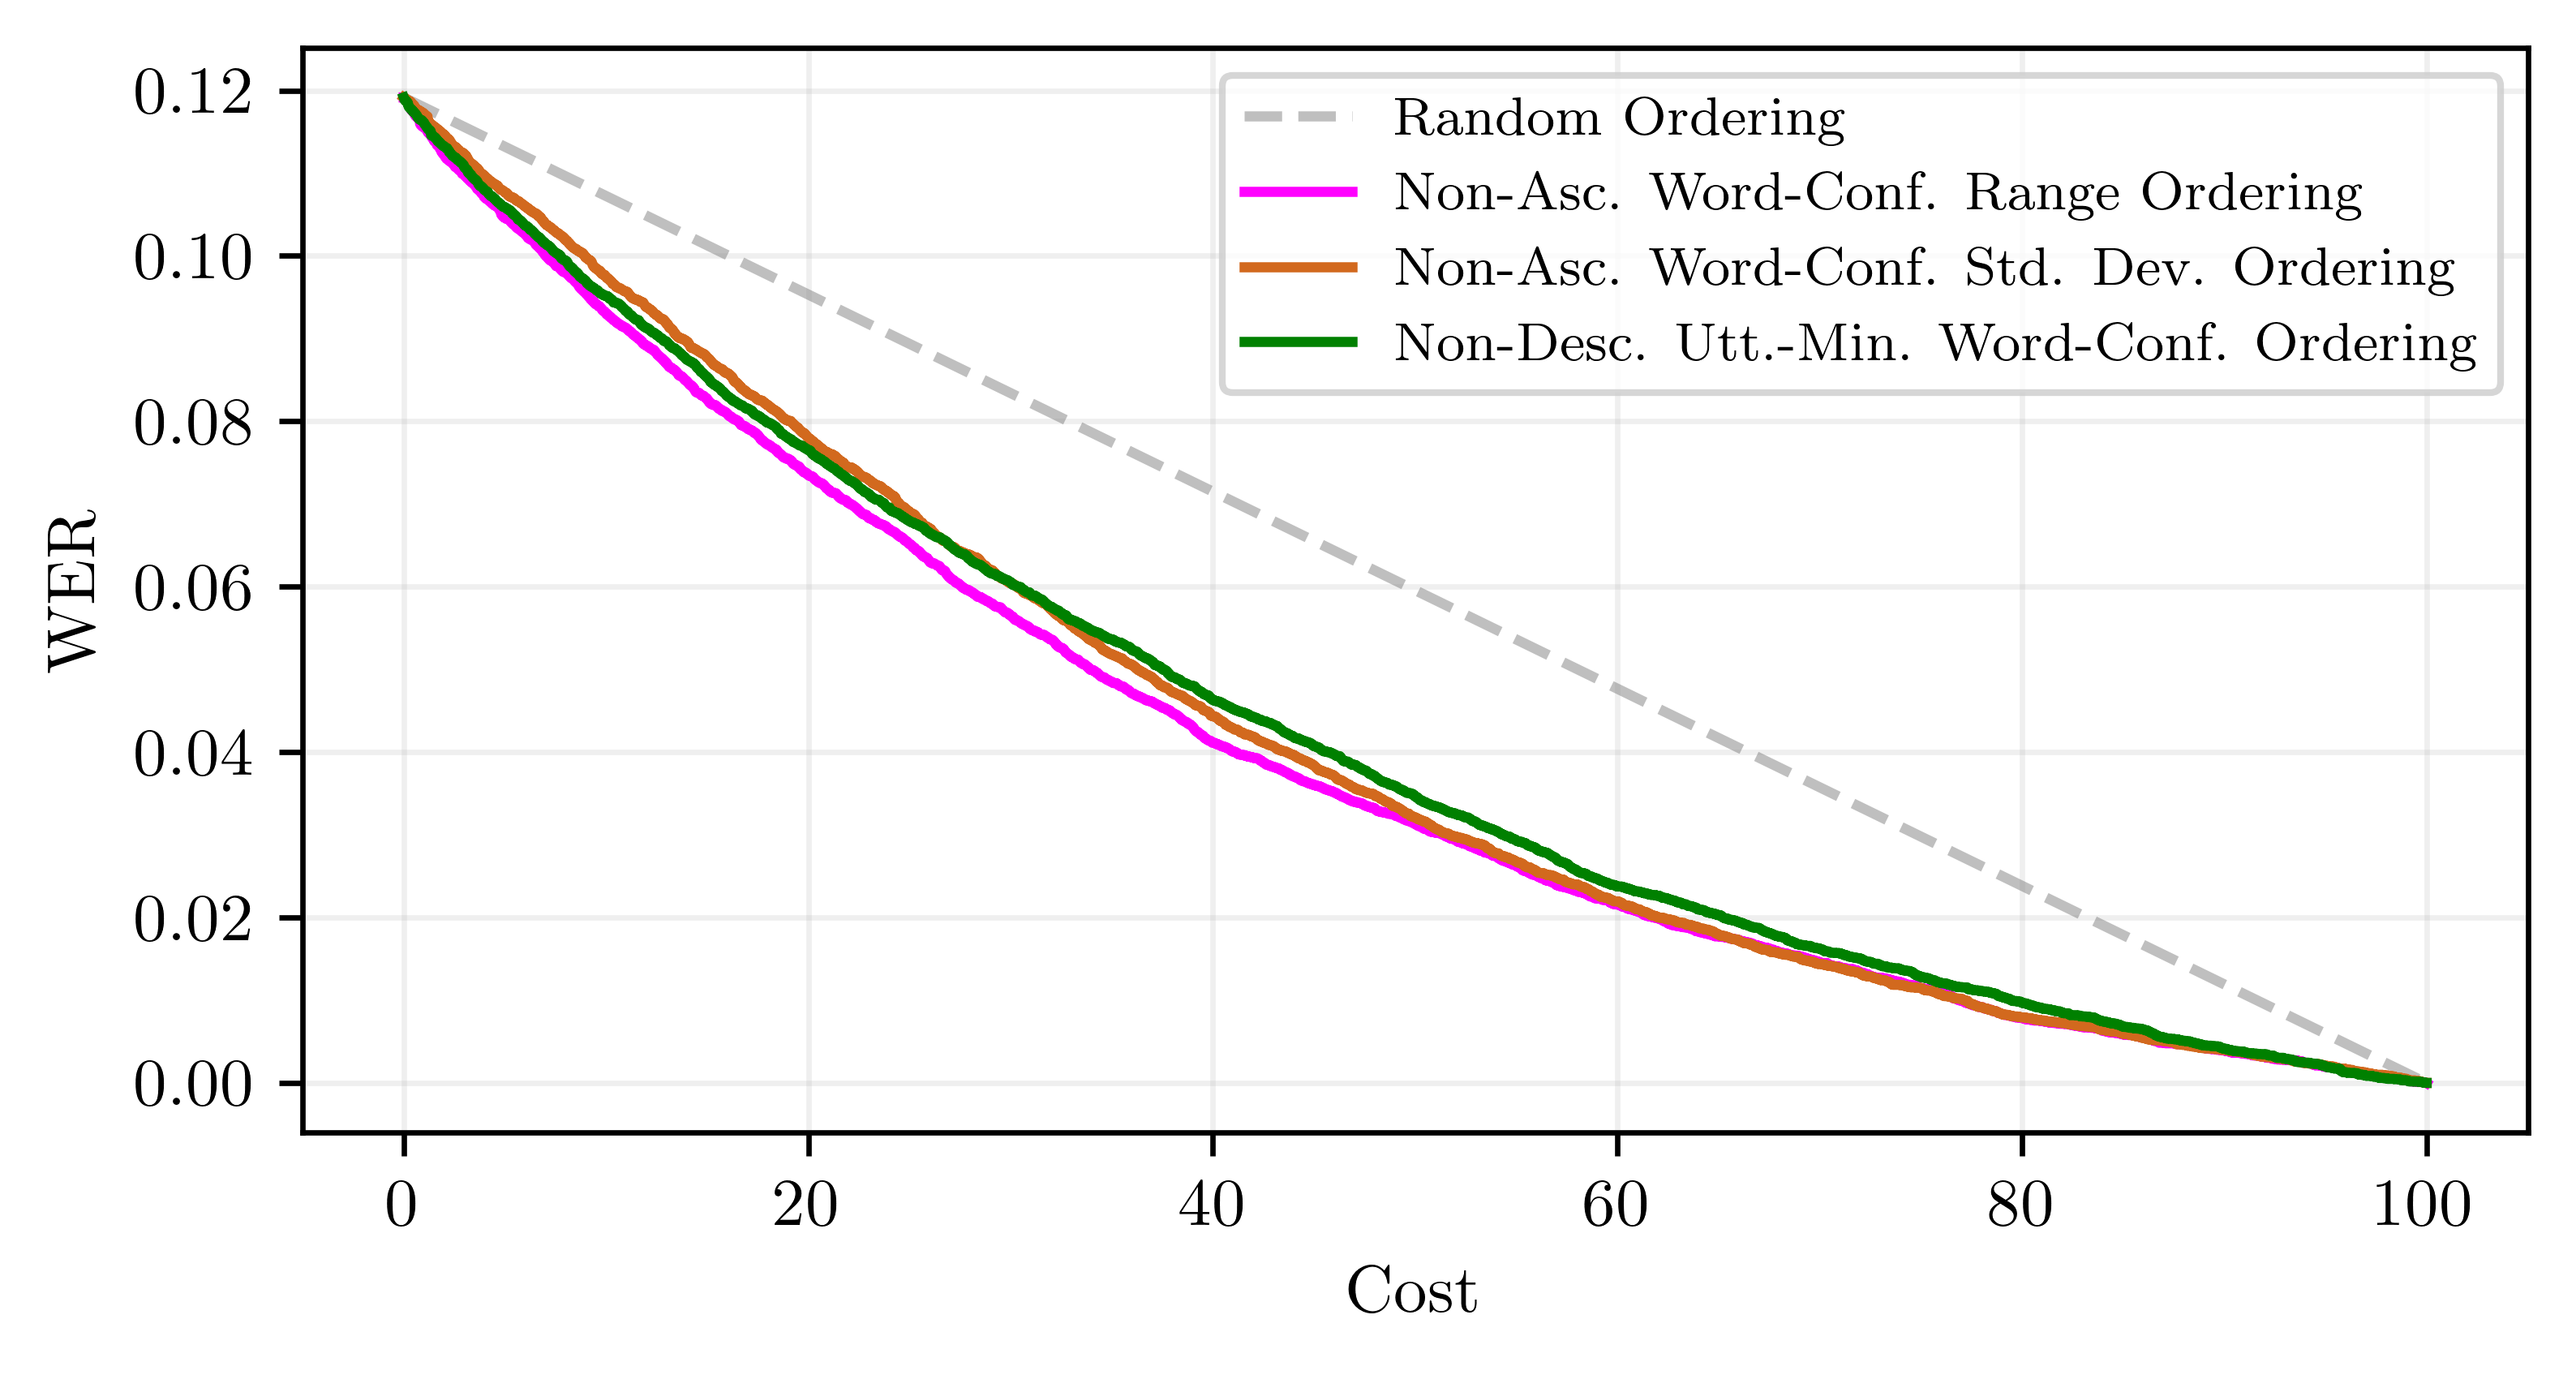
\includegraphics[width=\textwidth]{figures/range-ordering-vs-stddev-vs-min-wconf.png}
 \centering
\end{figure}
\begin{figure}[h!]
 \caption{WER difference between metrics and random ordering}
 \label{fig:delta-wer}
 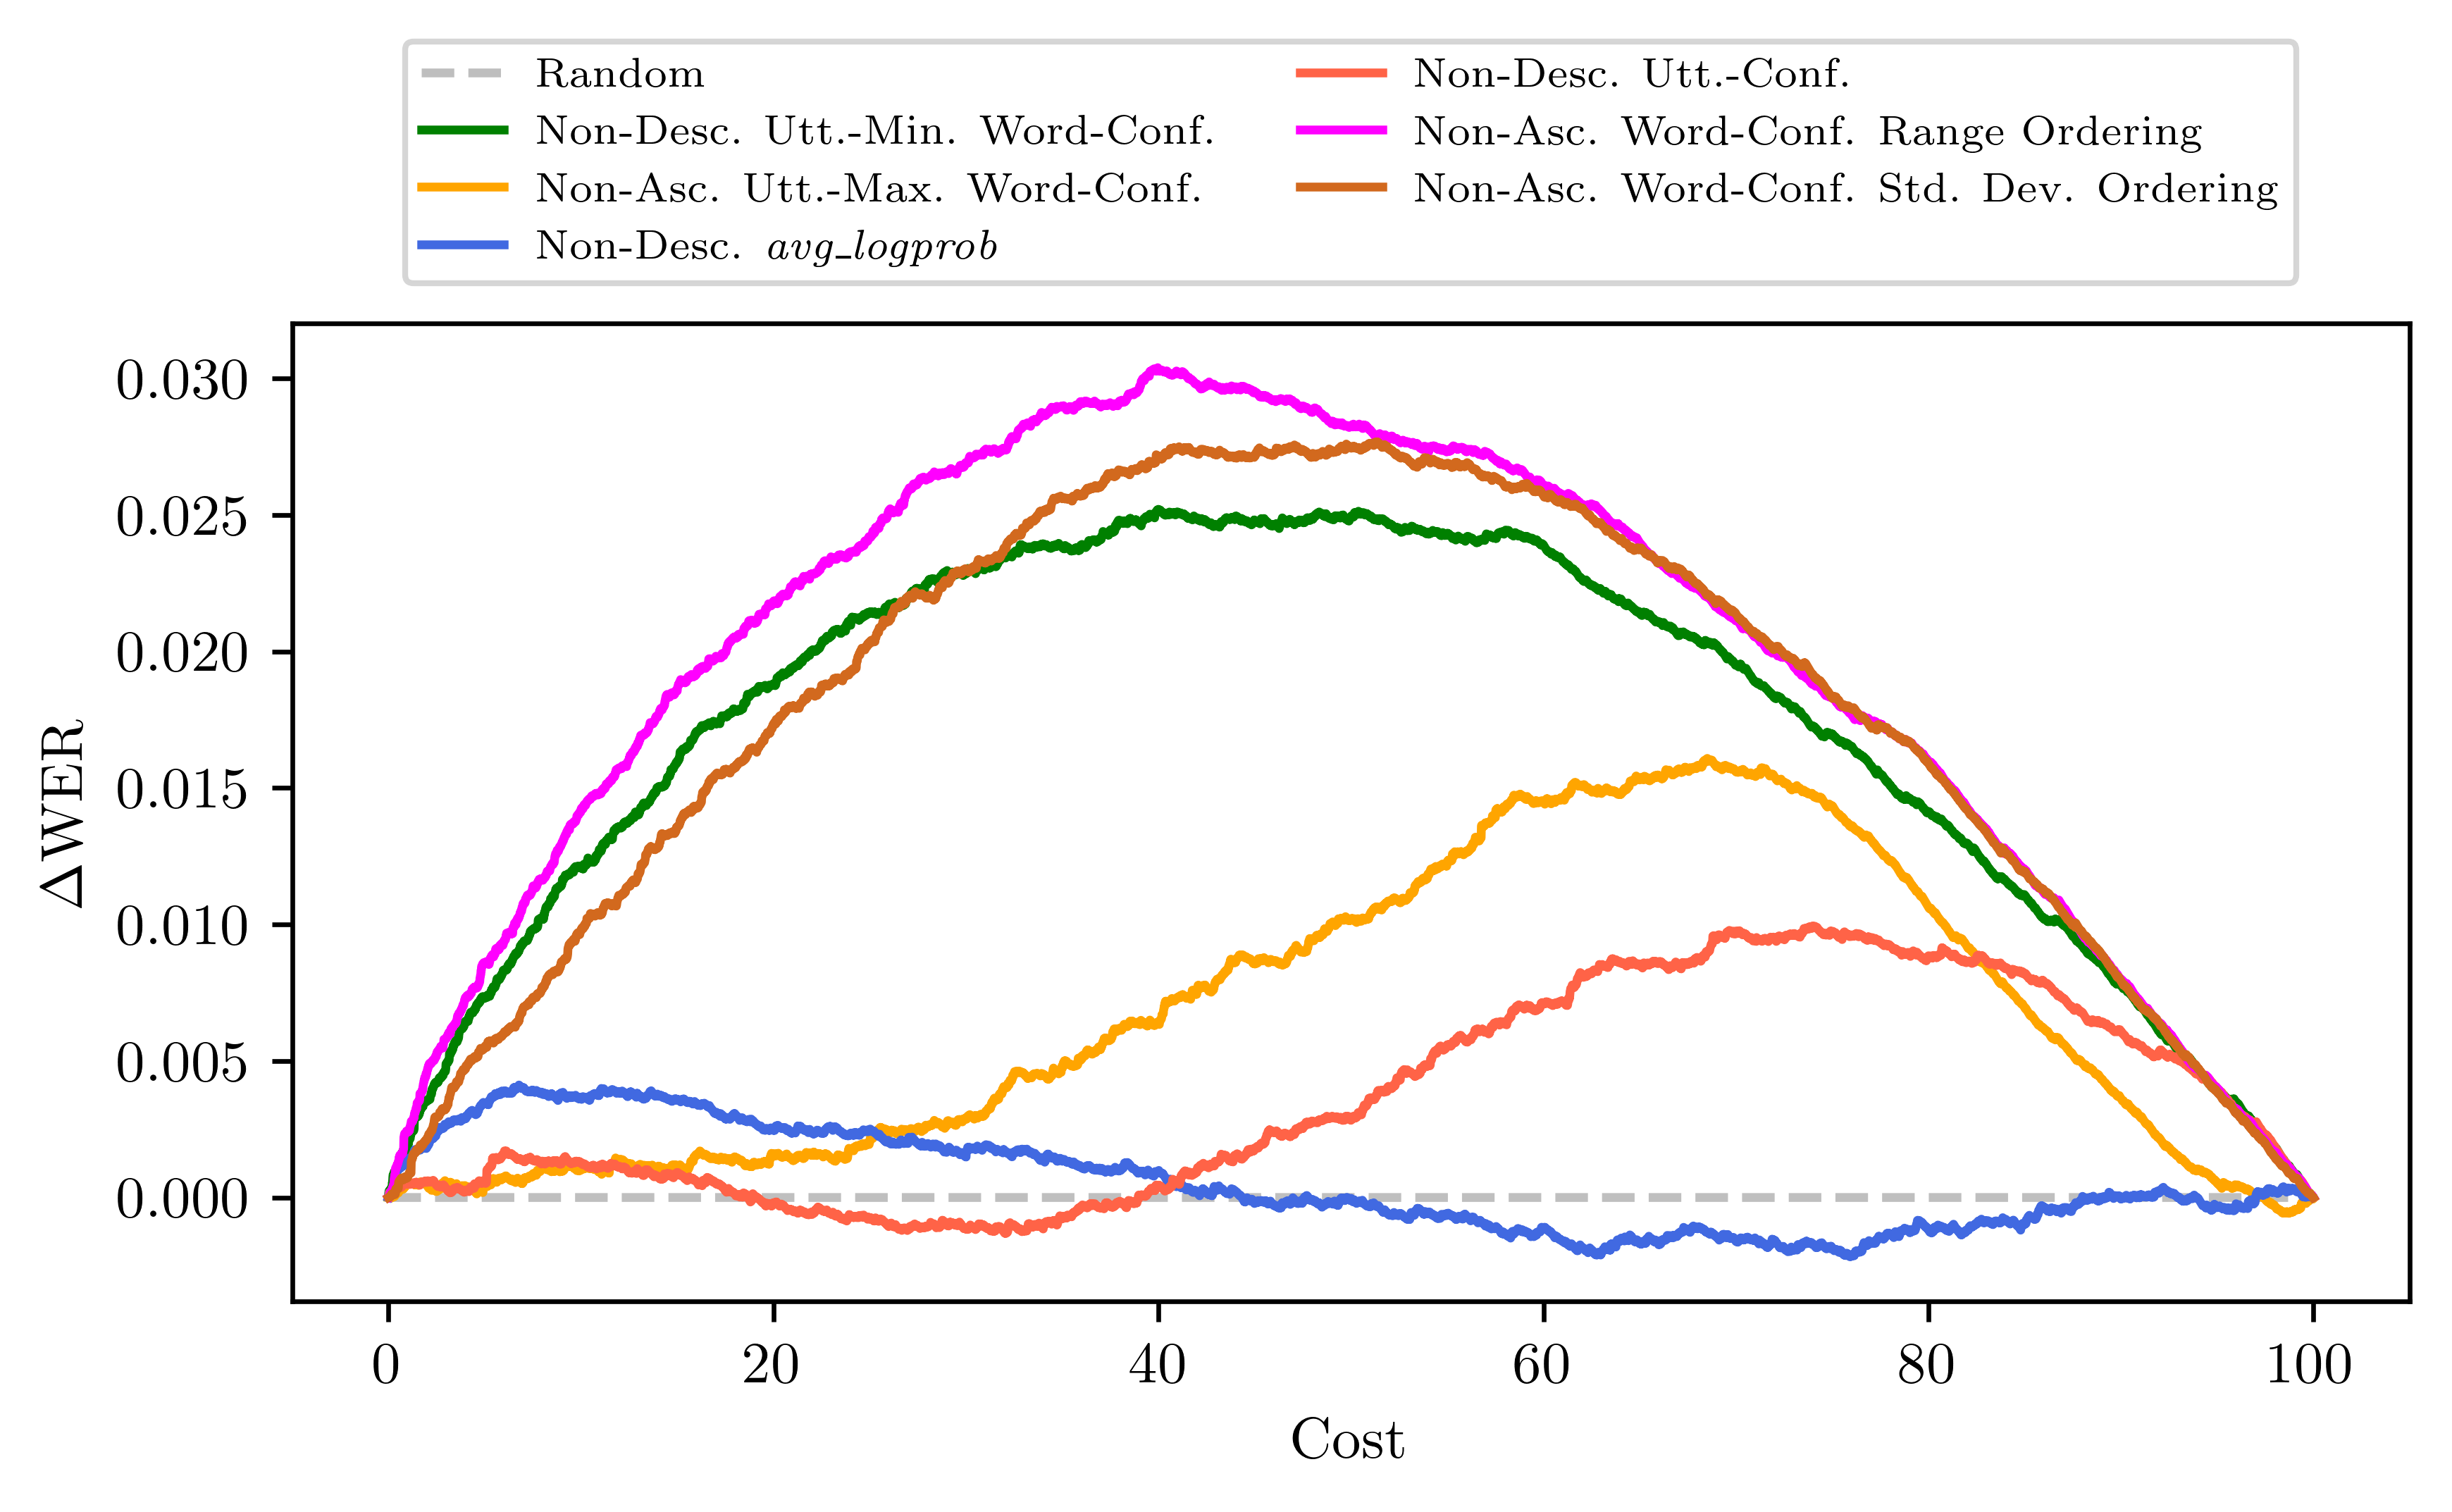
\includegraphics[width=\textwidth]{figures/delta-wer-all-allmeasures.png}
 \centering
\end{figure}




\clearpage
\section{Discussion of Results}

This section shall discuss findings which can be drawn from these results.

\subsection{Utterance-average confidence and \texttt{avg\_logprob}}

The results show that \texttt{avg\_logprob} and utterance-average confidence perform relatively similarly on average for a given conversation (fig. \ref{fig:compare-avg-uttconf-vs-lprob}), with similarly poor performance when used to order the entire corpus (fig. \ref{fig:corpus-avg-lprob-uttconf}).
Utterance-average confidence appears to have marginally superior performance in both comparisons shown in section \ref{subsec:avg-word-conf}.

\mycomment{
  need to explain how conf and lprob are calculated in implementation or design section
}
The similarity between the plots of the utterance-average word confidence and Whisper's \texttt{avg\_logprob} output is likely due to their similarity in calculation.
Confidence is calculated by \emph{whisper-timestamped}\cite{whisper-timestamped} from the average of the word-level confidence scores in an utterance, which are calculated from the average of the sub-word log-probabilities for each word.
Whisper\cite{whisper} calculates \texttt{avg\_logprob} as simply the average of the log-probabilities of all tokens in an utterance.
Perhaps the slight performance increase seen when using utterance-average confidence scores could be explained due to it being calculated from word-level scores rather than token-level and the accuracy metric operating at the word-level rather than token-level too.

\subsection{Word-level confidence metrics}

The results presented in section \ref{subsec:avg-word-conf} show the per-conversation average relationship between WER and Cost for the non-ascending and non-descending utterance-minimum and -maximum word-confidence metrics.

It is apparent that for the utterance-minimum word-confidence metric it is best to use non-descending (fig. \ref{fig:word-conf-comparison-plot1}) rather than non-ascending order (fig. \ref{fig:word-conf-comparison-plot2}), as non-ascending order closely follows the random order (i.e. is ineffective).
This makes intuitive sense because ordering results on non-ascending minimum confidence would mean correcting the most confident results first, thus the opposite of an effective ordering method.

Notice that non-descending utterance-minimum word-confidence ordering (fig. \ref{fig:word-conf-comparison-plot1}) has the narrowest shaded area of all the plots presented, meaning it has the lowest standard deviation from the mean and therefore the most reliable representation of performance on a given conversation.

As for using utterance-maximum word-confidence ordering, non-ascending order (fig. \ref{fig:word-conf-comparison-plot4}) shows superior performance to non-descending (fig. \ref{fig:word-conf-comparison-plot3}).
The reason for this is less intuitive; it would make more sense that ordering from lowest maximum confidence to highest (i.e. non-descending) would put utterances with lower confidence scores first.
This could be due to word-confidence being derived from word-level probability scores, though this is an area which needs more experimentation to better understand this result.

When comparing whole-corpus evaluation results using word-confidence measures (fig. \ref{fig:corpus-all-word-conf-measures}), non-descending utterance-minimum word-confidence ordering has the best (largest difference from random) and most consistent (smoothest line) performance of all the metrics, followed by non-ascending utterance-maximum word-confidence.
The other two metrics are shown to be a hinderance, achieving worse performance than if the results were evaluated in random order and should thus be ignored as metrics to use in a computer-aided transcription system.

\subsection{Comparing word-level and utterance-level metrics}

Figure \ref{fig:corpus-allmeasures} presents a comparison between the performance of each metric when evaluating the whole corpus.
The metric with the best performance is clearly non-descending utterance-minimum word-confidence; it is much more consistent than the others and remains much further from random ordering, meaning it has the highest WER reduction for the same cost as all other metrics.

Figure \ref{fig:range-ordering-vs-stddev-vs-min-wconf} shows the performance of non-ascending ordering using the both range scores and standard deviation of word-confidence for each utterance. 
Notice the slight performance gains over non-descending utterance-minimum word-confidence.
When ordering utterances using the best performing metric, non-ascending word-confidence range, checking only 40\% of the results gives a relative reduction in WER of over 65\% compared to not checking any ASR-generated results.

% Please add the following required packages to your document preamble:
% \usepackage{booktabs}
\begin{table}[p]
\centering
\begin{tabular}{@{}rl@{}}
\toprule
\multicolumn{1}{l}{\textbf{Utterance Ordering Metric}} & \textbf{\begin{tabular}[c]{@{}l@{}}Cost to reduce\\WER by 50\% \end{tabular}} \\ \toprule
Random                                                                                      & 50.0\%          \\ \midrule
\begin{tabular}[c]{@{}r@{}}Non-descending utterance-minimum \\ word-confidence\end{tabular} & 30.7\%          \\ \midrule
\begin{tabular}[c]{@{}r@{}}Non-ascending word-confidence\\  range\end{tabular}              & \textbf{27.9\%} \\ \midrule
\begin{tabular}[c]{@{}r@{}}Non-ascending word-confidence \\ standard deviation\end{tabular} & 30.6\%          \\ \midrule
  Non-descending \texttt{avg\_logprob}                                                                   & 50.1\%          \\ \midrule
Non-descending utterance-confidence                                                         & 47.7\%          \\ \midrule
\begin{tabular}[c]{@{}r@{}}Non-descending utterance-maximum\\ word-confidence\end{tabular}  & 43.2\%          \\ \bottomrule
\end{tabular}
  \label{table:halve-wer-results}
  \caption{Cost required to halve WER.}
\end{table}


These metrics show slight performance gains over non-descending utterance-minimum word-confidence, though these gains are best illustrated in figure \ref{fig:delta-wer}, which plots the difference in WER from using random ordering ($\Delta$WER) against Cost.



\section{Future Work}

This section shall suggest areas which may benefit from further work in the future which have become clear while completing this work.
